\begin{figure*}
  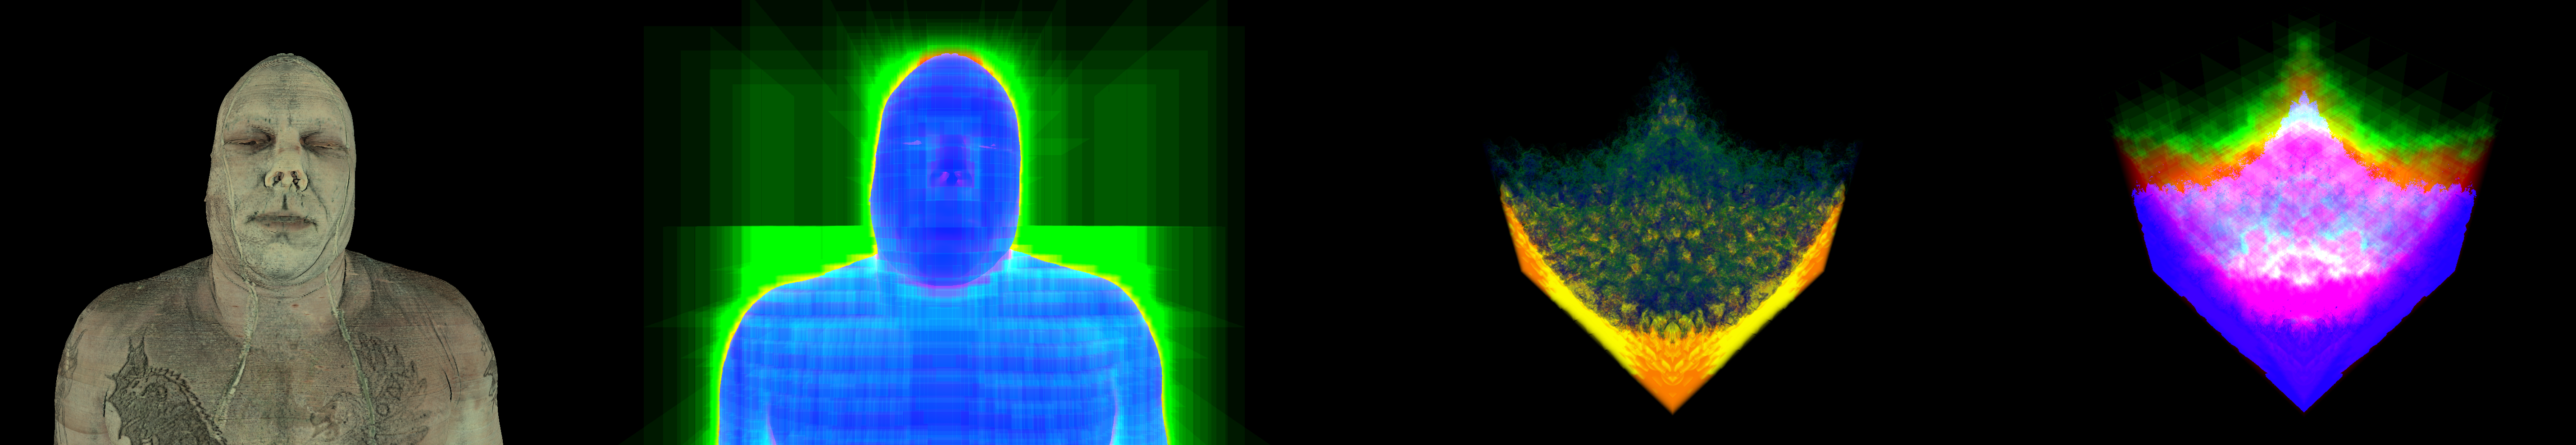
\includegraphics[draft=\isDraft, width=1.00\linewidth]{images/rg/teaser.png}
  \caption{The Visible Human male full color (\tjftilde{}12~GB) and
  a Richtmyer-Meshkov instability (\tjftilde{}8~GB) render in 34~ms
  and 58~ms, respectively, using our ray-guided volume rendering
  implementation.  On right are views which highlight the areas
  that take advantage of empty space leaping (green) and early ray
  termination (blue).}
  \label{fig:teaser}
\end{figure*}

\section{Abstract}
Volume rendering continues to be a critical method for analyzing
large-scale scalar fields, in disciplines as diverse as biomedical
engineering and computational fluid dynamics.
% On the one side,
% ever-increasing scanner capabilities has resulted in the proliferation
% of datasets with vastly increased resolution.  On the other, massive
% parallel supercomputing resources has enabled simulations at
% unprecedented resolutions.
Commodity desktop hardware has struggled to keep pace with data
size increases, challenging modern visualization software to
deliver responsive interactions for $O(N^3)$ algorithms such as
volume rendering.  We target the data type common in these domains:
regularly-structured data.

In this work, we demonstrate that the major limitation of most volume
rendering approaches is their inability to switch the data sampling
rate (and thus data size) quickly.  Using a volume renderer inspired by
recent work, we demonstrate that the actual amount of visualizable data
for a
scene is typically bound \emph{considerably} lower than the memory
available on a commodity GPU.  Our instrumented renderer is used to
investigate design decisions typically swept under the rug in volume
rendering literature.  The renderer is freely available, with binaries
for all major platforms as well as full source code, to encourage
reproduction and comparison with future research.

\section{Introduction}

Modern volume rendering is heavily focused on the concepts of empty
space skipping and the fast detection of ray saturation.  Both of
these concepts have extensive effects on the amount of compute work
required.  However, even more relevant is their ability to reduce the
working set of extremely large datasets down to a small kernel, which
can significantly reduce the amount of data which must be loaded from a
slow resource, such as the network or a local disk.  This has enabled
interactive volume rendering for very large data on commodity
hardware~\cite{Knoll:2010:BVH, Hadwiger:2012:Guided,
Crassin:2009:Gigavoxels}.

There are a variety of trade-offs in the development of a modern volume
renderer.  The choice of brick size, for example, can significantly
impact the effectiveness of empty space skipping.  We note that the
presentation of most volume rendering systems lacks detailed insight
into these parameters.  Further, these factors can interact in complex
ways.  As an example, empty space skipping works considerably better
with smaller bricks sizes, but disk throughput drops sharply with small
requests.  Compression can further complicate the issue.

We seek to rectify this situation by performing a thorough study of
the interaction of these parameters within the context of GPU-based
ray driven volume rendering.  We have surveyed recent volume rendering
literature and implemented a renderer by piecing together the best
ideas from a multitude of systems. These ideas were extended with
notions required for our environment---for example, by removing
the requirement that datasets fit in GPU memory.  Along the way,
we instrumented every corner of the renderer and utilized this
instrumentation to exhaustively explore relevant options.  The final
result achieves better performance than previous work and provides a
guided tour through the maze of design choices available in a modern
volume renderer.

\begin{figure*}
  \centering
  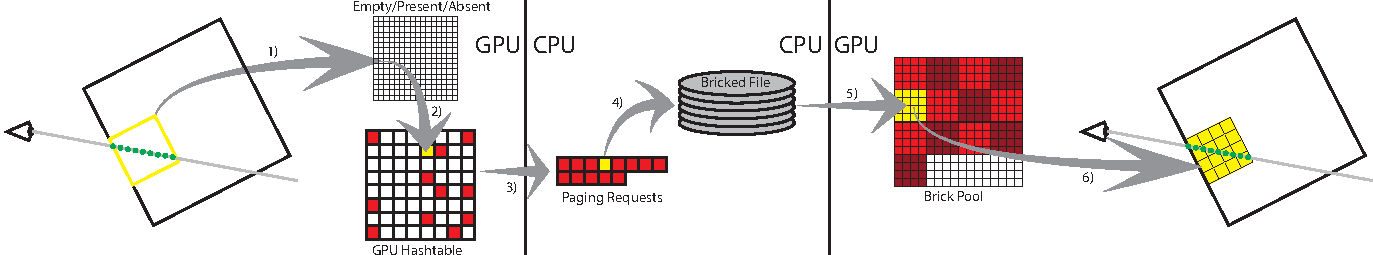
\includegraphics[width=1.00\linewidth]{images/rg/pipeline.pdf}
  \caption{The missing brick reporting / paging subsystem of our volume
  rendering approach.  Missing bricks are recorded into a hash table
  (1, 2), to be paged in (3, 4, 5) and rendered in subsequent frames
  (6).}
  \label{fig:flow}
\end{figure*}

\section{Related Work}

Volume visualization on consumer graphics hardware has become widely
utilized as a means to cope with the growing sizes of data.  GPUs have
proven useful in both ray-tracing and rasterization
techniques~\cite{Reichl:2012:HybridSurface, Dick:2009:Terrain},
rendering of diverse scenes~\cite{Parker:2010:Optix}, as well
as considerably more general tasks~\cite{Owens:2007:GPGPU}.

Volume rendering accelerated by GPU hardware was established in the
mid-90's~\cite{Cullip:1993:AVRW, Cabral:1994:AVRA}, initially based on
hardware compositing of volume slices.  The ability to do raycasting
came later~\cite{Krueger:2003:ATGV}.  Since the time of the initial
GPU-based volume renderers, researchers have been concerned with
methods to work around the limited memory available on GPUs.  The
prominent technique for volume rendering large data on a GPU is to use
a multiresolution
representation~\cite{Boada:2001:Multires, LaMar:2000:Multires,
Weiler:2000:LoD}.  This method hinges on the concepts of empty space
leaping and early ray termination~\cite{Levoy:EarlyTermination}, two
techniques developed early on which demonstrate that sampling can be
significantly reduced in many instances of volume rendering.

There has been much work on accelerating ray-traced volume rendering in
recent years.  Voreen implements a more general architecture,
including GPU-based raycasting~\cite{Voreen:2009}.  Tuvok implements a
flexible volume rendering system with support for very large
datasets~\cite{Fogal:2010:Tuvok, Fogal:2009:SizeMatters}.  Knoll et al.
utilize a bounding volume hierarchy and optimized SSE to achieve very
fast
volume renderings~\cite{Knoll:2010:BVH}.  Gobbetti et al. and Boada et
al. detail methods for traversing tree structures on the GPU for
the purpose of volume rendering~\cite{Gobbetti:2008:VR,
Boada:2001:Octree}.
The Gigavoxels~\cite{Crassin:2009:Gigavoxels} system traverses
$N^3$-trees on the GPU to choose an effective resolution.  With the
large gap between processing power and data sizes, some communities
have turned to distributed memory systems for large-scale
volume rendering~\cite{Childs:2006:ScalableVR, Howison:2010:MPIHybrid,
Fogal:2010:HPG, Beyer:2012:DSM}.

Our algorithm employs a lock-free data structure on the GPU for
feedback information.  Highly-concurrent Lock-free structures are ideal
for the manycore GPU environment, however they have previously been
challenged by the lack of concurrency primitives available for the
OpenGL platform.  We make use of a lock-free hash table very similar to
that of Michael's~\cite{Michael:2002:LockFreeHT}, implemented in a
manner similar to Lux and Fr\"ohlich's implementation for terrain
rendering~\cite{Lux:2011:RCHeight}.

Hadwiger et al. presented a volume renderer similar to
ours~\cite{Hadwiger:2012:Guided}.  Their system is aimed at volume
rendering highly anisotropic data as it is streamed real-time from a
high-resolution microscope.  Our renderer improves upon theirs in a
number of ways:

\begin{itemize}
  \itemsep0em
  \item We perform brick lookup each brick, instead of every sample,
  maintaining the simple and familiar ray-marching core that is
  well-documented in volume rendering literature.

  \item We expound on how to use modern GPU features to implement our
  lock-free feedback data structure, which enables the implementation
  to spend more time computing on the GPU and less time pushing data
  around.

  \item We utilize an out-of-core, progressive rendering methodology,
  breaking the GPU-memory-size barrier that limits data sizes from
  Hadwiger et al.'s work.  This also allows us to gracefully scale down
  to consumer-level graphics cards.
\end{itemize}

While we believe these to be novel additions, we do not consider them
to be this work's major contribution.  Rather, we provide new depth to
the discussions of a variety of parameters which are relevant in the
development of a ray-guided direct volume renderer:

\begin{itemize}
  \itemsep0em
  \item The strategy to be used to load higher resolution data when a
  variety of intermediate choices are possible;

  \item an understanding of the miasma of issues surrounding bricking
  and brick sizes;

  \item empirical evidence demonstrating that the working set for
  direct volume rendering is indeed bound more by the screen resolution
  than the dataset;

  \item a novel method for ray-guidance storage and propagation to the
  input system's logic;

  \item how to effectively handle real-time updates to the transfer
  function; and

  \item the effect of brick layout strategies on large volume access
  times.

\end{itemize}

% improvements upon gigavoxels:
%  . we don't require a hierarchy (but of course one can be used)
%  . they use MRTs to store their information on which brick is
%    needed.  this (a) wastes their MRTs, of which one only has 8
%    on modern GPUs, and (b) means that their memory for doing
%    this is extremely limited.  since we use image_load_store,
%    our HT for storing this is decoupled from the actual
%    rendering, and can scale up (or down) arbitrarily

In contrast to previous renderers, ray-guided volume renderers couple
the rendering process with the identification of which subvolumes
(`bricks') must be loaded.  We describe the operation of ray-guided
volume renderers, in Section~\ref{sec:algorithm}.
In Section~\ref{sec:performance} we detail a plethora of benchmarks
which demonstrate the performance of the renderer.

In many prior volume renderer evaluations, results are generally
limited to the raw performance of the renderer.  However, we note
that---for some reason---users of our volume renderer rarely ask how
many milliseconds it takes
to render the visual human.  One thing users \emph{do} ask is how large
the data can get before the renderer becomes unusable. For this reason,
we have engineered our renderer so that it does not require that the
volume fit in core.  Furthermore, users generally value a responsive
system over a performant system.  They are curious if money should be
spent upgrading a video card or buying a solid state drive.  Design
elements are carefully expounded and conclusions are drawn in
Section~\ref{sec:tradeoffs}.

Finally, Section~\ref{sec:conclusion} gives our final remarks, and note
both limitations and opportunities for future work.

\section{Ray-Guided Grid Leaping}
\label{sec:algorithm}

At the macro level, our algorithm is reminiscent of the recent work of
Hadwiger et
al. ~\cite{Hadwiger:2012:Guided}, as well as Engel's
CERA-TVR~\cite{Engel:2012:CERA} which in turn is based on the
Gigavoxels
system~\cite{Crassin:2009:Gigavoxels}.

With Hadwiger et al., we share the requirement of a set of simple
multiresolution Cartesian grids, along with an OpenGL-based table
to report missing bricks.  A multiresolution hierarchy is built as a
preprocess for input data which exist at only one resolution (details
are in Section~\ref{sec:tradeoffs}).  From the CERA-TVR system
we inherit the idea to only recompute and request grid cells at
boundaries.

\subsection{Overview}

We endeavor to create a volume renderer which can render massive 
datasets extremely fast on commodity GPU hardware.  The major issues in
such a renderer are:
\begin{enumerate}
  \itemsep0em
  \item Identifying regions which must be sampled densely.

  \item Precisely locating the transition between these regions and
  regions which exhibit considerable homogeneity.

  \item Terminating a ray as soon as possible.

  \item Efficiently communicating regions to be rendered in the future
  to the IO layer.

\end{enumerate}

Points (1) and (2) ensure we concentrate the computational effort on
the areas which require it.  Point (3) is critical because it means we
do not have to load the data beyond the point of early termination,
significantly reducing costly disk traffic.  If point (4) is not
sufficiently addressed, the renderer will load large amounts of data
which are not needed for rendering, at severe costs in performance.

% new subsection header here? we are switching from properties a
% Ray-guided VR needs to how we implemented said properties, here

To the first point, we employ an efficient metadata structure which
allows us to quickly identify these regions.  Points (2) and (3) are
handled through an educated choice of brick size, which is discussed
more thoroughly in Section \ref{sec:tradeoffs}.  A major component to
modern volume renderers is how they address point (4), now by and large
based on \emph{ray guidance}.  That is, the sampling characteristics of
the ray determine which data to load.  Stated differently, the future
data requirements are computed \emph{in concert} with standard ray
traversal and accumulation.

% \todo{here we might want to say something about how regular disk I/O
% is in modern volume renderers, and allude to a later section where we
% discuss data organization}

The entire operation is detailed in Figure \ref{fig:flow}. For each
ray we compute the level of detail required to maintain a pixel error
of less than one. With this level and the position in the volume we
compute a brick index.  This brick index is used to fetch information
from a lookup table
(Figure \ref{fig:flow}.1) to identify whether the brick is a) empty, b)
non-empty and present on the GPU, or c) non-empty and absent. When it
is empty, we skip the brick and repeat the process at the brick's exit
point.  When it is non-empty and present, we ray-cast that brick. When
the brick is non-empty \emph{and} not resident in GPU memory, the
system returns the finest coarser level available and the missing entry
is added to a GPU hash table (Figure
\ref{fig:flow}.2). This table is read back to the host memory at the
end of the frame (Figure \ref{fig:flow}.3), and used to page in bricks
from
disk or cache (Figure \ref{fig:flow}.4).  A paged-in brick is then
uploaded to a GPU texture pool
(Figure \ref{fig:flow}.5), and a subsequent frame will use this
portion of the brick pool for sampling (Figure \ref{fig:flow}.6).

% While we do not require a full hierarchy---only that coarser versions
% of the data exist---we generate a multiresolution hierarchy for such
% data as a preprocess.

The key component is that both ray-accumulation \emph{as well
as} identification of the bricks which are needed should occur
on the GPU.  The latter is natural to compute during standard
ray-casting operations.  Doing both operations on the GPU means brick
identification comes very cheap, as it parallelizes very effectively.
More importantly, performing this during ray-casting ensures that it
is optimally accurate: the program never loads data which will not be
used.

%---we get results which are as accurate as the brick size.

\begin{algorithm}
  \caption{Ray-guided volume rendering.  Each ray identifies the
  set of bricks which it needs for rendering independently, and
  reports this information for use in subsequent rendering passes.}
  \label{alg:vrender}
  \begin{algorithmic}[1]
%  \If{$rayResumePos = FINISHED$} \Return \EndIf
  \State \textit{color} = \textit{rayResumeColor}
  \State \textit{terminated} = \textbf{true} \Comment{assume ray will finish}
  \Repeat
    \State \textit{LoD} = ComputeLOD(Depth(\textit{ray}))
    \State \textit{brick, samplingRate} = GetBrick(\textit{ray})
    \State \textit{offsets} = PoolOffsets(\textit{brick})
    \If{\textit{samplingRate} $\neq$ RequiredSamplingForLOD(\textit{LoD})}
      \State ReportMissingBrick(\textit{brick})
      \If{\textit{terminated}} \Comment{\emph{first} missing brick?}
        \State \textit{terminated} = \textbf{false}
        \State \textit{rayResumePos} = \textit{ray}
      \EndIf
    \EndIf
    \State Raycast(\textit{ray}, \textit{stepSize}, \textit{offsets})
  \Until{\textit{ray} $\geq$ \textit{exit} $\lor$ Saturated(\textit{ray})}
  \State \textit{rayResumeColor} = \textit{color}
  \If{\textit{done}}
    \State \textit{rayResumePos} = \textbf{FINISHED}
  \EndIf
  \end{algorithmic}
\end{algorithm}

The basic algorithm is given in Algorithm \ref{alg:vrender}.  Briefly, the
appropriate sampling rate is identified and we look for the data at
that resolution (lines 4, 5).
\texttt{GetBrick} will always return some data, but the data may be at
a lower resolution than request; this is
communicated through the \texttt{stepSize} and the situation is handled
on line 7.  If our data are too coarse, we note that we are missing a
brick (\texttt{ReportMissingBrick}) and where we are in the volume
(\texttt{rayResumePos}) when
this \emph{first} occurred (\texttt{terminated}).

% A key insight is that the relationship between \texttt{GetBrick} and
% multiresolution data can be entirely opaque.  The function simply
% takes a region and returns a chunk of memory to be ray-traced, with
% information as to how it should be sampled.  In stark contrast to the
% Gigavoxels system, a strict hierarchy is not required, and indeed our
% system does not organize data on the GPU in this manner.

% \begin{algorithm}
%   \caption{Ray-casting inner loop.  Operation is equivalent to a
%   traditional ray-casting volume renderer, with the minor addition
%   of offsets into the volume pool.  Checking in the outer loop is
%   sufficient and allows this core inner loop to stay simple.}
%   \label{alg:inner-loop}
%   \begin{algorithmic}[0]
%     \While{$ray \not\geq$ Exit($brick$)}
%       \State $v =$ sampleVol($ray$ + $offsets_{pool}$)
%       \State $c =$ TransferFunction($v$)
%       \State $color = color + (1 - \alpha) \times c$
%       \State $ray = ray + stepSize$
%     \EndWhile
%   \end{algorithmic}
% \end{algorithm}

Every iteration through the outer loop, we perform this identification
of the appropriate resolution.  This satisfies our first goal as
mentioned above: we identify the appropriate sampling resolution
at every brick boundary.  With small bricks, this means we will do
few integration steps before early ray termination is recognized.
Furthermore, we detect empty bricks at this stage as well.
% and so we will sample no more data than a single brick before
% recognizing empty space.

% The \texttt{Raycast} function is listed in Algorithm
% \ref{alg:inner-loop}.  Note that this is equivalent to `standard'
% ray-casted volume rendering in more traditional volume renderers,
% sans the minor addition of \texttt{offsets} when sampling the
% volume data.  In fact, this is not a unique aspect of our renderer;
% any renderer which uses a volume pool would share this code.  The
% simplicity of the volume rendering loop is a prime benefit to our
% approach; the entire GLSL core consists of less than 600 lines of code,
% including all the debugging and profiling targets used to generate
% images and timing results for this paper.

% \subsection{Mixed Levels of Detail}
% 
% As the sampled resolution can differ at arbitrary points along the ray,
% a natural concern is what sampling methodology is required to ensure
% these boundaries are not visible in the rendering.  In this section, we
% demonstrate empirically that no advanced sampling schemes are required.
% 
% The appropriate sampling rate for a given region of space is a function
% of the frustum settings and the depth of the current sampling position.
% The depth is the only parameter which varies
% \emph{while} we progress along a ray.  Moreover, the appropriate
% sampling rate is aliased to the relatively few levels of detail which
% are available for a dataset.
% 
% \begin{figure}
%   \centering
%   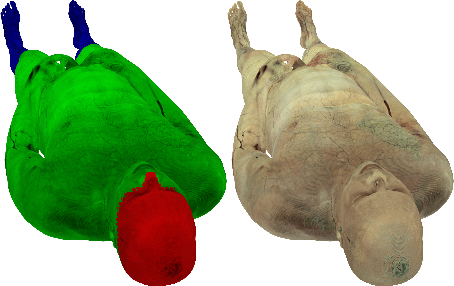
\includegraphics[width=\linewidth]{images/simultaneousLoDs-1}
%   \caption{Volume rendering of the full color visible human dataset
%   with color-coded levels of detail.  It is difficult to derive viewing
%   conditions for which a plethora of LoDs are required; the relatively
%   few LoDs visible here come from an extreme case.}
%   \label{fig:LODs}
% \end{figure}
% 
% In practice, even for highly anisotropic data, it is difficult to
% derive frustum and viewing angles which result in the simultaneous
% visibility of more than three levels of detail.  Figure
% \ref{fig:LODs} demonstrates this: as the ray switches from one level
% of detail to another, the color is flipped---bricks rendered at the
% highest resolution for the viewpoint are in red, and the lowest
% resolution data has a blue tint.  Looking at these areas side-by-side,
% it is clear that such boundaries are not visible in normal volume
% renderings.
 
%% this was moved to a single sentence at the beginning of sec:algorithm
% \todo{This paragraph feels really out of place here, but we need something
% similar \emph{somewhere} (reviewer comment)} Of course, many volume
% datasets are not provided in a multiresolution form.  For such data,
% we generate multiresolution representations as a preprocess.  This need
% only be done once, of course, and is relatively fast: 72 minutes on
% a modern Intel i7 machine for a typical case, the Richtmyer-Meshkov
% instability (`RMI', $2048x2048x1920$ voxels).  We note, however, that
% this process scales very poorly with the brick size: small brick sizes
% take considerably more time. More
% discussion is provided in Section~\ref{sec:tradeoffs}.

% or 5391.92 seconds / 60 = 89.87 minutes on a Xeon

\subsection{Missing Data}

As noted above, it is possible that data are undersampled while
rendering.  When this occurs, we display a coarser version of the data
initially, but progressively refine those regions with finer resolution
data until they are sampled at a rate of a single voxel per pixel, or
the maximum data resolution available.  This information is collected
by the GPU as it renders, but must be communicated back to the CPU to
coordinate disk access and update the appropriate area of the volume
pool.

One solution for this would be to use multiple render targets to store
information on which bricks are missing~\cite{Crassin:2009:Gigavoxels}.
The limitation of this method is the limited mapping operation from
the ray to the target buffer: there are only so many available render
targets.
Furthermore, this approach ignores the inherent spatial coherency
between rays.  Two neighboring rays are highly likely to request the
same set of bricks, or at least have substantial overlap within the
sets they require.  With the multiple render targets approach, both
pixels will encode the same value, and we will need to read back larger
textures which consist of predominantly duplicate values.

Instead of utilizing extra render targets, we take advantage of an
OpenGL extension which was promoted to core in version 4.2,
\texttt{GL\_ARB\_shader\_image\_load\_store}.  This extension allows
the creation of an image buffer which is independent of the current
rendering buffer.  Using the atomic load/store operations the extension
provides, we implement a set based on a linearly-probed lock-free hash
table stored in an \texttt{image\_load\_store} buffer.  Since we are
hashing based on the brick, multiple rays requesting the same brick hash
to the same position.  This allows us to keep the table---and therefore
how much information we read back per-frame---quite small.  We discuss
sizing of the hash table in more detail in
Section \ref{sec:ht-params}.

\begin{figure}[t]
  \centering
  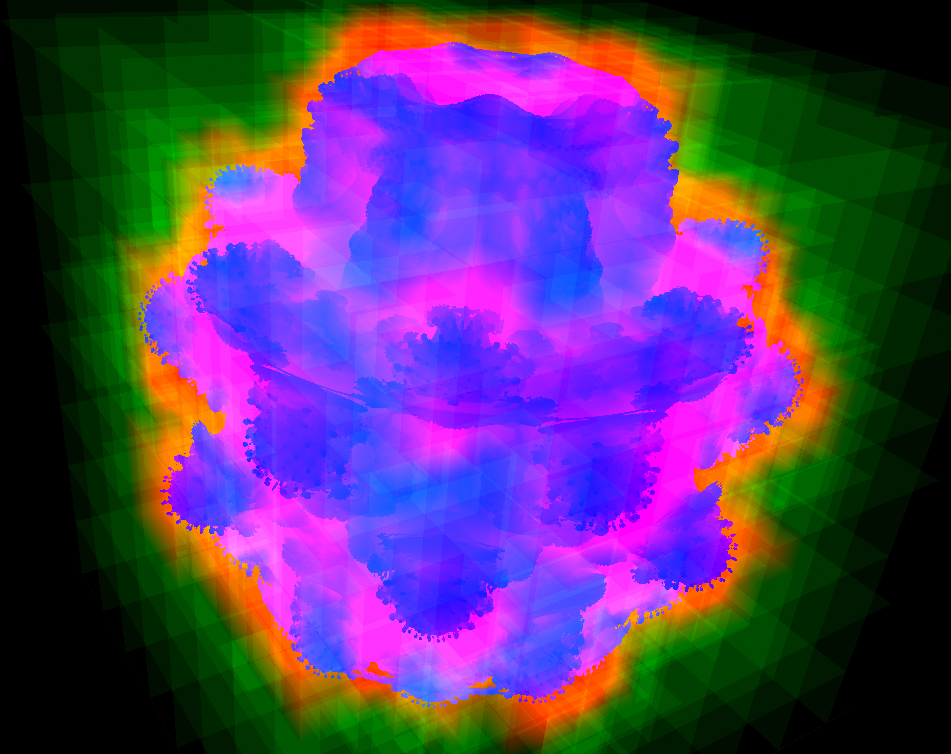
\includegraphics[width=0.95\linewidth]{images/rg/terminate-empty.png}
  \caption{Volume rendering behavior for the Mandelbulb dataset.
  Green indicates bricks which were skipped via empty space skipping.
  Red indicates bricks which were sampled densely.  Blue indicates
  bricks which were sampled but saturated quickly.
%  Most rays skip almost all of the data or terminate very quickly;
%  the lack of white regions in this rendering indicate that, here,
%  \emph{all} rays fall into a single category.
  }
  \label{fig:bricks-empty}
\end{figure}

\begin{figure*}
  \centering
  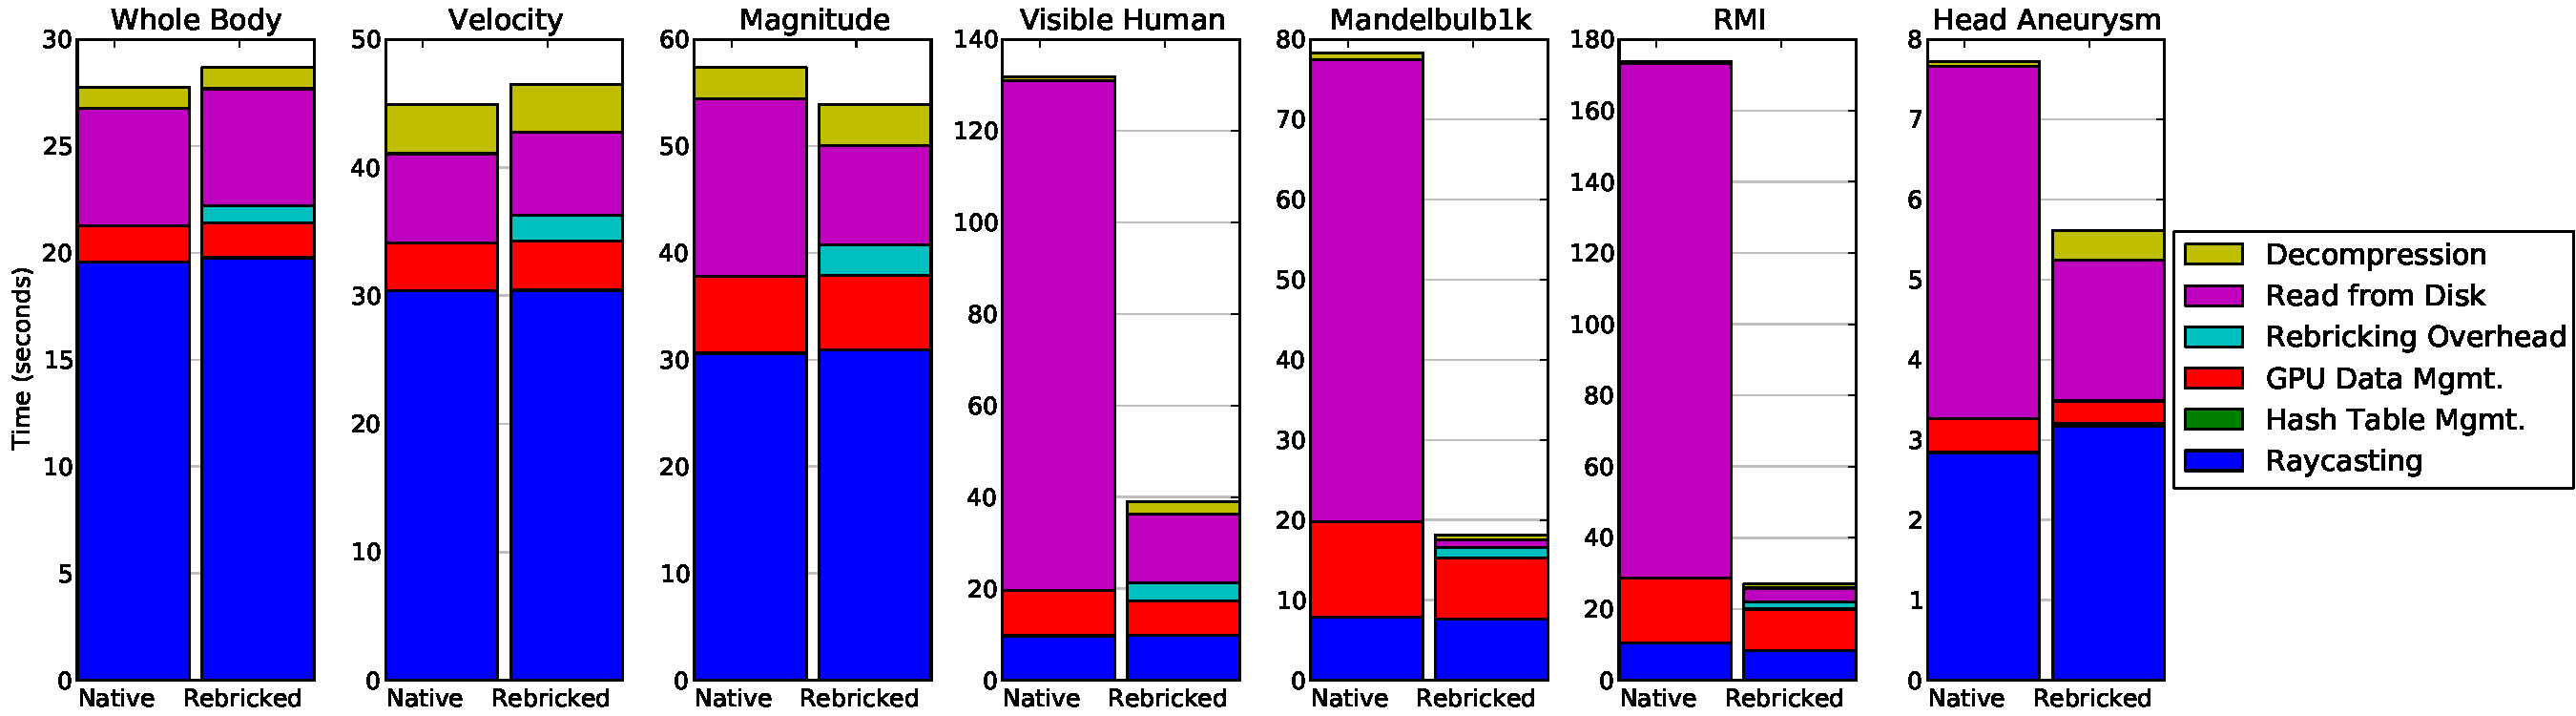
\includegraphics[width=1.00\linewidth]{images/rg/breakdown.pdf}

  \caption{Time spent at various stages of our pipeline, aggregated
  over the generation of a rotation sequence.  Comparisons are made
  between data stored with the ideal brick size for that dataset
  (`Native'), and data stored at a large brick size of $256^3$ with
  the ideally-sized bricks created at run-time (`Rebricked').  `Whole
  Body', `Velocity', and `Magnitude' suffer from a lack of ray
  saturation.}

  \label{fig:breakdown}
\end{figure*}

\subsection{Brick Classification}
\label{sec:brick-classification}

Considering our target goals (1) through (3) given at the beginning of
this section, one could classify a brick into one of three categories:
\begin{itemize}
  \itemsep0em
  \item skipped due to empty space skipping,

  \item early termination due to ray saturation, or

  \item sampled densely without saturating.
\end{itemize}

An important observation is that---in a very large number of
cases---bricks fall into \emph{either} the `empty' or `saturating'
categories, and only \emph{rarely} in the `non-saturating' category.
The factor which has the greatest effect on performance is how quickly
a renderer can classify data into one of the first two categories, and
therefore bypass a large set of the work.

To make this identification effective, ray-guided volume renderers
maintain the state of each brick, shared on both the GPU and host
memories.  During rendering, one uses the table to identify if a brick
is empty.  If so, the renderer leaps over that space instead.  We store
this as an array consisting of one 32-bit integer per brick of the
dataset.

Figure \ref{fig:bricks-empty} visualizes this classification for a
large dataset under a typical view and transfer function.  As shown
there, the majority of the visualization falls into either the `blue'
(saturated quickly) or `green' (skipped) sets. This also demonstrates
how little data is actually required for a typical volume rendering.  A
similar rendering is given in the rightmost image of
Figure \ref{fig:teaser}, in which only the rays in the middle of the
volume require high computation.

Of course, this classification depends largely on the transfer function
and viewing parameters.  In practice, however, transfer functions which
produce \emph{informative} visualizations tend to exhibit such ternary
classifications.

When the transfer function is changed, this metadata information
must be recomputed.  For datasets with many bricks, this can induce
a noticeable delay.  Our current test platform can process about
7.5 million bricks per second, but even a 1 second delay between
interactions is too much.  Therefore, we offload this update to a
background thread.  Until the thread completes its work, the renderer
considers all unprocessed bricks to be `missing', causing it to request
bricks which might be empty.  Those bricks' metadata is directly
updated and they are only loaded if they fail the empty check.  The
overall performance effects may be large, but the system remains
responsive during this period.

\section{Performance}
\label{sec:performance}

In this section, we give an overview of the various stages of the
renderer and how they perform.  Unless otherwise noted, all timings
were performed on a dual quad-core Xeon 2.2~GHz system using an NVIDIA
GeForce GTX 680, with 24~GB of system memory and 4~GB of GPU memory.
We mostly report results from commodity hard drives, explicitly noting
some specific relevant uses of SSDs.  In many cases, results were
obtained from multiple screen resolutions, but we report results from
an HD viewport ($1920\times1080$) unless noted otherwise.  Details of
the data utilized and renderer timings are given in
Appendix~\ref{sec:data}.

\subsection{Benchmarks}

We have chosen a variety of benchmarks to evaluate the performance of
our renderer, and we elucidate the logic behind those choices here.
First, the choice of HD resolution is motivated by voxel-to-pixel error
ratios.  All modern high-performance volume renderers try to maintain a
1-to-1 ratio between projected voxels and pixels.  Adaptive resolution
selection is used to ensure this ratio.  Without this feature, results
will be aliased, too much information will be compressed to a single
pixel, and performance will suffer.  Adaptive resolution means that
small viewports will not stress renderers: a 512$\times$512 viewport
can get along fine with a paltry few hundred megabytes of memory,
irrespective of the input dataset size.

We utilize zoom-ins, as in the accompanying video and results such as
those in Figure~\ref{fig:working-set} and some in
Table~\ref{tbl:timings}, to accentuate these high resolution issues.
When the volume is far away, a very coarse resolution is utilized which
maintains accurate voxel-to-pixel error ratios.  As the camera comes
closer, higher resolutions of the source data must be utilized.  We
terminate zoom-ins slightly after they fill the screen; beyond this
point, frustum culling's effect dominates (see
Figure~\ref{fig:working-set}).  The most challenging cases for a
volume renderer are when data are close enough to be seen at native
resolution, but far enough away that no data can be culled by the
frustum.

Rotations are used to demonstrate that the renderer does not rely
solely on early ray termination.  As described in
Section~\ref{sec:brick-classification} and depicted in
Figure~\ref{fig:bricks-empty}, most rays either skip large parts of
the volume, or terminate very quickly.  With a transfer function that
produces a dense volume, bricks in the front will prevent bricks in the
rear from ever being paged in, effectively meaning the volume renderer
need only cope with the front \emph{half} or even less of the volume.
Barring pathological volumes and transfer function choices, rotations
ensure all of the data has a chance to contribute to a sequence.

\paragraph{Transfer functions.} Changing a transfer function is also
an important benchmark in any volume rendering system.  Doing so
invalidates our brick metadata concerning which bricks are empty,
causing some hash table entries in the next frame to make little sense
(i.e. request bricks which are visible under the old transfer function
but empty under the new one).  Furthermore, the bricks in the GPU
volume pool may be inappropriate for the new transfer function.

Renderer performance as measured by response time during such an
interaction actually changes very little, and can even improve.
However, quality suffers rather drastically.  This is evident in the
time to convergence after a change in the transfer function: in a
typical case with the RMI data set (see Section~\ref{sec:data}), time
to convergence increased over 6x after changing the transfer function
(from $\sim$380ms to $\sim$2300ms).

\begin{figure*}
  \centering
  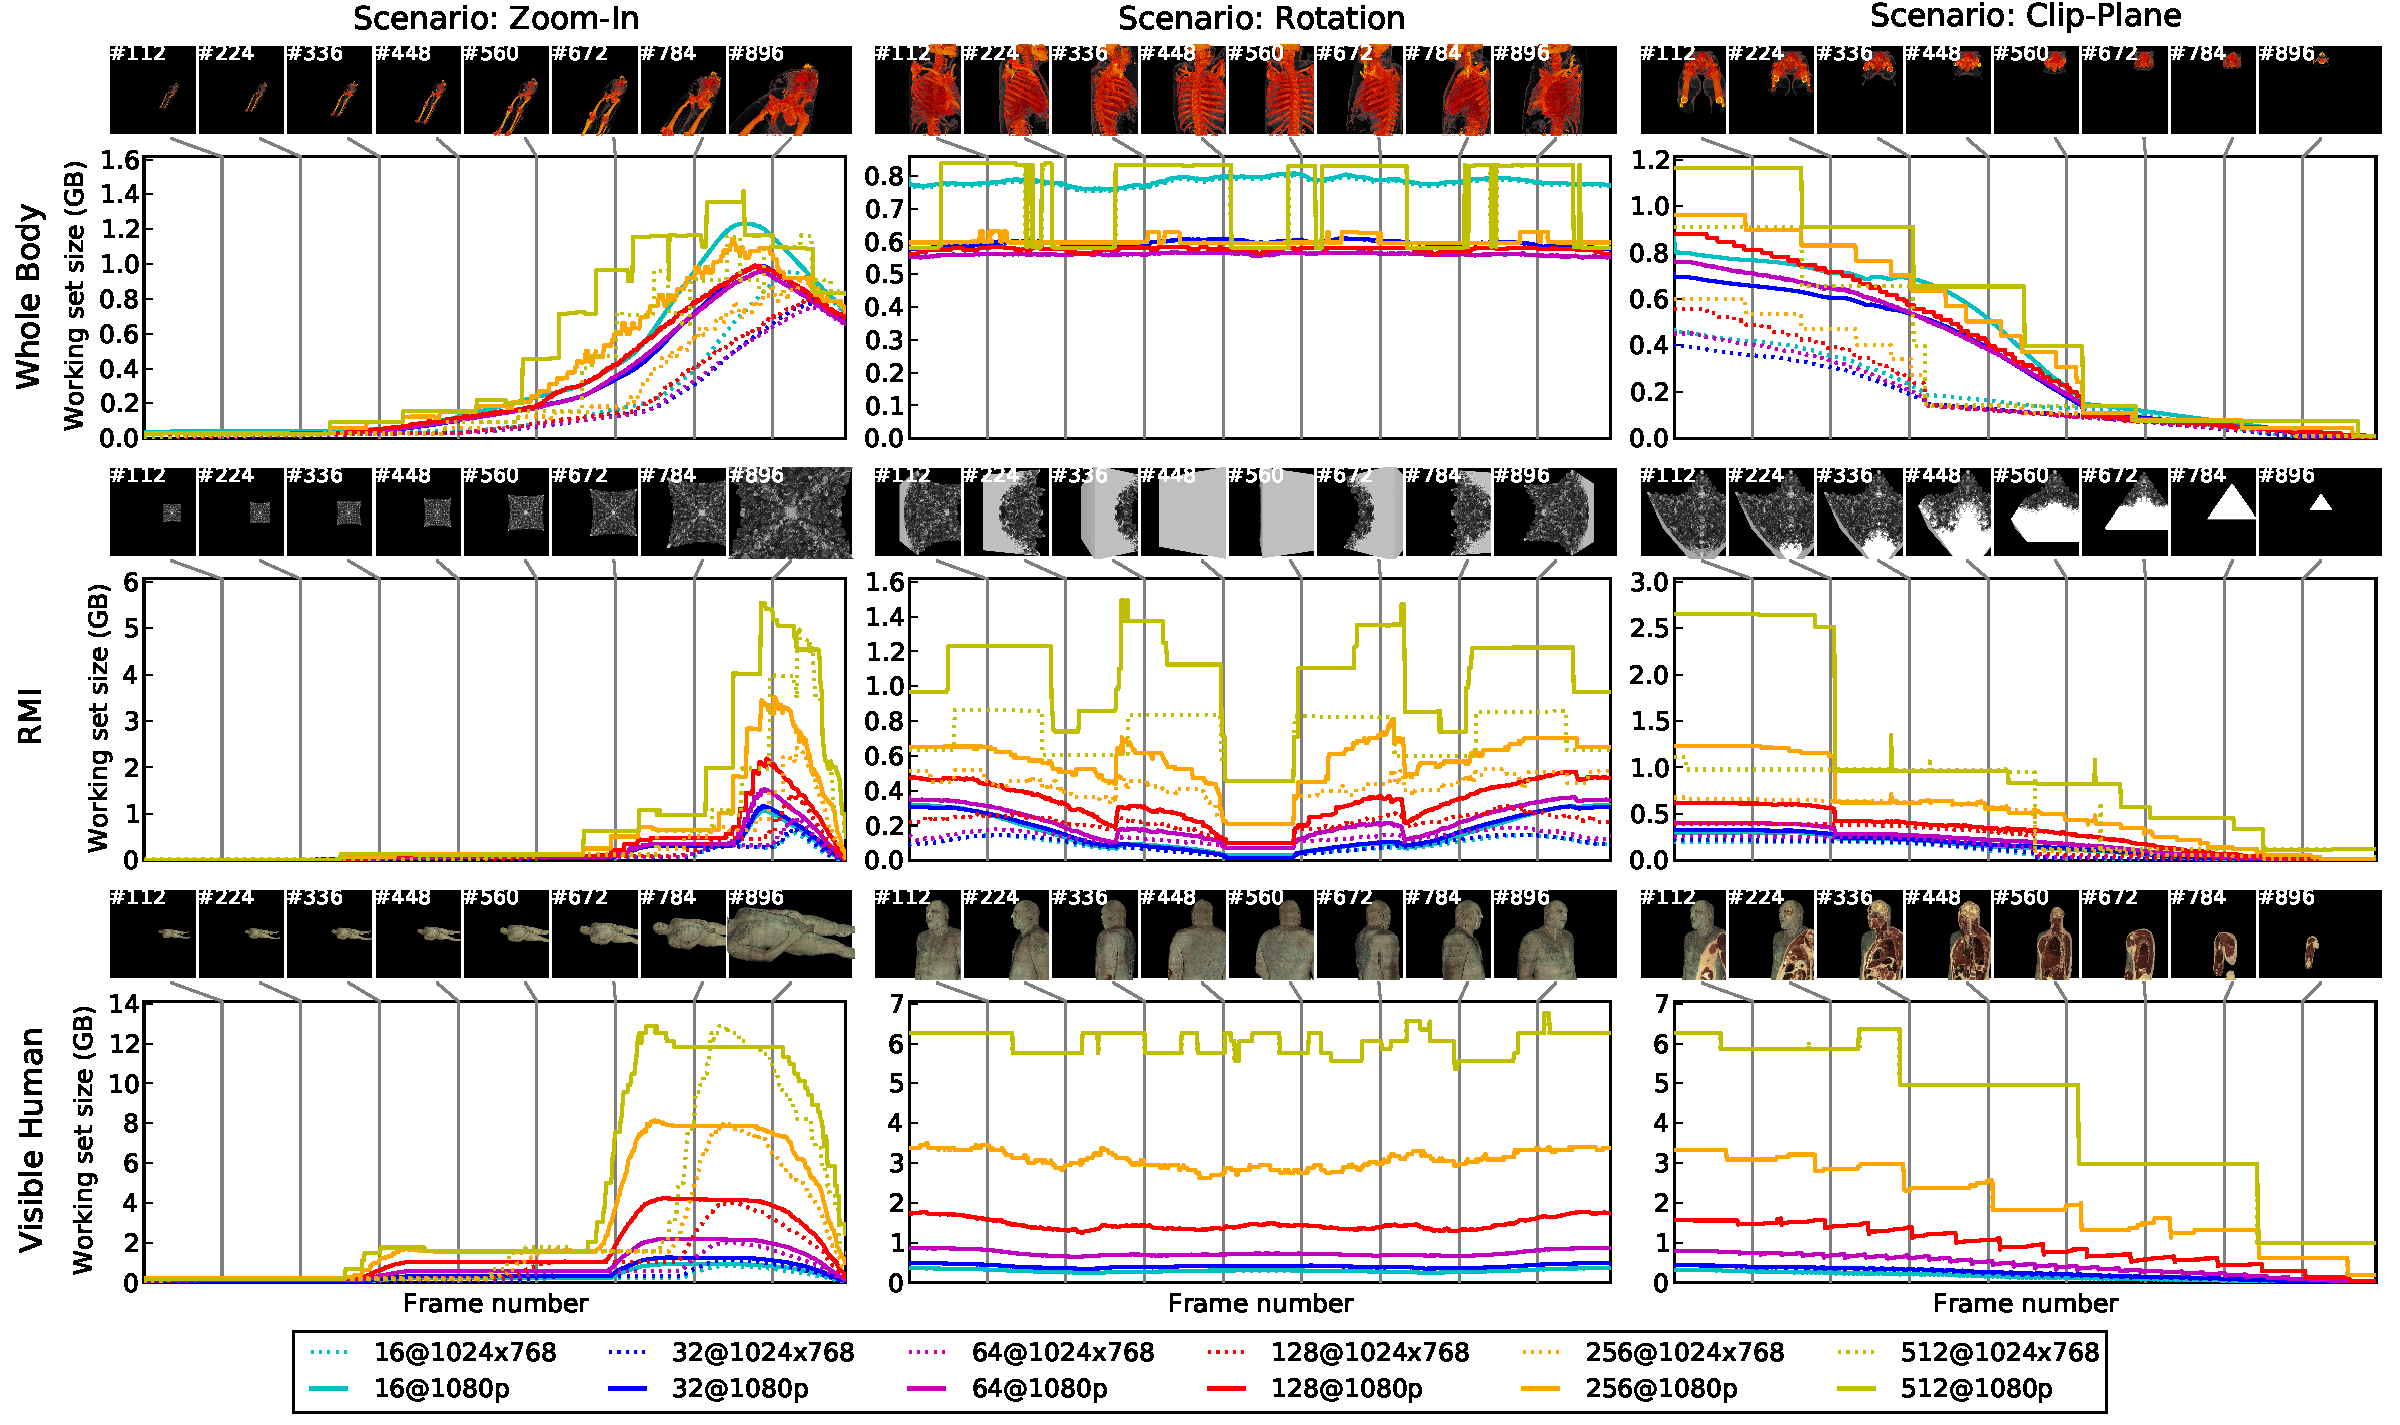
\includegraphics[width=0.98\linewidth]{images/rg/workingSets1-150dpi.pdf}
  \caption{Working set sizes across three different scenarios for
  multiple datasets.  Smaller brick sizes approximate the working set
  better.}
  \label{fig:working-set}
\end{figure*}

\subsection{Results}
\label{sec:results}

To evaluate our renderer in different scenarios, we used a standard
rotation scenario with a variety of datasets, measuring the length of
each pipeline stage.  Figure~\ref{fig:breakdown} has these results.  As
IO is the prime bottleneck in many cases, we implemented a `rebricking'
scheme to mitigate the amount of IO performed.  Using large reads and
caching, this significantly lowers the time spent doing IO.  We used
`LZ4' compression when recording this performance data, which trades
CPU time for IO time.

The majority of the time is spent ray-casting, pulling data from disk,
and uploading the bricks to the pool.  Our novel hash table approach
keeps the table small, and so reading it is very cheap: even for large
data, this component does not factor in to the overall performance.
The other GPU data to manage is metadata information for our volume
pool (i.e. which bricks are resident), but at a single machine word per
brick it costs very little to push it down to the GPU, even for very
large data.

Interestingly, the time spent managing GPU data is an increasing
function of volume size \emph{until} it peaks around the size of the
RMI ($2048\times2048\times1920$).  This reinforces our assertion that
there is only so much data visible in a given frame---dependent only on
the view
frustum, and \emph{not} the dataset size---and so at some point we
saturate the set of visible data.  Figure~\ref{fig:working-set} and
Section~\ref{sec:subdivision} include more discussion about working set
sizes.

% \todo{datasets to beat/compare with:
% 2048x1024x1080, 16bit, 640x480 viewport: 95 minutes to preprocess
% ($32^3$). biomedical data (lizard scan?).  12 to 30 Hz range; avg 16 Hz
% for volume rendering, avg 20 Hz for
% iso. dvr had peak memory use of: 153.125 megabytes\cite{Gobbetti:2008:VR}.\\
% 21494x25790x1850, 1024x768 viewport. ``mouse cortex''. two transfer
% functions: one runs at 75 Hz, another at 12.\cite{Beyer:2012:DSM}\\
% 18000x18000x304, 1024x768 viewport.  77 Hz and 19
% Hz\cite{Beyer:2012:DSM}.\\
% $2048^3$, 1024x768 viewport.  55 and 30 Hz.\cite{Beyer:2012:DSM}.
% }

\section{Design Tradeoffs}
\label{sec:tradeoffs}

In this section, we try to explore aspects which have not been
thoroughly addressed by previous literature.  Details on trade-offs and
the reasoning behind our final implementation choices are given.

% There are a variety of considerations in a ray-guided volume renderer
% which have not been thoroughly addressed in previous literature.  We
% endeavor to explore some of these choices here, and explicitly detail
% the inherent trade-offs and reasoning behind our final decisions.

\subsection{Subdivision}
\label{sec:subdivision}

How a system subdivides the volume into manageable pieces can have
a large effect on the performance of the renderer.  The primary
considerations are in regard to early ray termination and empty space
skipping: small bricks are much more likely to be composed of a small
range or even uniform values, which will make it more likely that the
brick can be skipped under a large set of transfer functions.  Further,
small bricks means one will detect ray saturation much more quickly, as
this is checked only when exiting a brick.

\paragraph{Internal Overhead}

The primary drawback is reduced disk throughput due to utilizing many
small requests.  A further drawback is the data size overhead: each
brick needs two voxels of ghost data in each dimension, for sampling
and gradient computation purposes.  This is negligible for large
bricks, but grows sharply as the brick size approaches one, as shown in
Figure
\ref{fig:brick-size}. Figure~\ref{fig:hierarchy-build} demonstrates
that this is not strictly a theoretical result: a small brick size
greatly increases not just size overhead, but also the time to
reorganize the data on disk.  From these Figures we can derive that for
large datasets a brick size of less than $16^3$ is impractical.

\paragraph{External Overhead}

We have performed a number of experiments to identify the working set
size for multiple different brick sizes.  Starting with the smallest
practical size of $16^3$, we increase the brick size up to $512^3$.

As can be seen in Figure~\ref{fig:working-set} the working set is bound
not by just the data size, but the screen resolution as well.  It can
also be seen that the brick size heavily influences the working set
size: larger bricks allow for less efficient utilization of empty
regions. From the images we can derive that a brick size of less than
$128^3$ is desirable to reduce the working set to roughly the memory
size of a GPU.

We note that the working set size is not a strict function of the brick
size, however.  Figure~\ref{fig:working-set} and
Table~\ref{tbl:timings} also show that the choice of brick size is not
clear-cut.  The Visible Human male performs best with $16^3$ bricks,
for example, whereas the ideal brick size for the `Magnitude' data is
$64^3$.  For the `Whole Body' dataset, using brick sizes of
$16^3$ actually resulted in \emph{larger} working sets than $32^3$.
This occurs when the transfer function produces large regions
of semi-transparency but never reaches saturation.  Indeed, when datasets
contain large swaths of semi-transparent regions, the conventional
wisdom is reversed: large brick sizes are generally preferred, since
they significantly improve disk throughput.

% \paragraph{Performance}
%
% There are three primary metrics to be concerned with when evaluating
% a volume renderer's performance.  One of them is the commonly
% evaluated metric: the time required to render the data at the
% required resolution.  The second is system responsiveness: if the
% user changes a viewing parameter, a transfer function, or any other
% state, the renderer should respond quickly.  A third consideration is
% the time to generate these data: converting a large dataset into a
% bricked representation grows sharply as the brick size shrinks.
%
% \todo{table or graph of brick size (X) and `time to build hierarchy' (Y)}

%% moved this up into other paragraph
% As can be seen Table \ref{tbl:timings} and Figure
% \ref{fig:working-set}, the brick size choice is not clear-cut.
%   The
% Visible Human male performs best with $16^3$ bricks, for example,
% whereas the ideal brick size for the `Magnitude' data is $64^3$.  When
% the transfer function keeps large regions mostly transparent, as is the
% case for the `Whole Body' and `Velocity' datasets, then the improved IO
% performance gleaned from large requests derives the most benefit.

If we begin to consider secondary metrics, such as the response time of
the system, the choice of brick size becomes even more complex.  Since
bricks are the atomic building blocks in a volume renderer, one cannot
load less than a single brick from disk. Therefore a larger brick size
imposes a larger response time on the system.  These concerns would
generally push a designer to choose smaller bricks.

However, disk performance falls very sharply with small
requests~\cite{Fogal:2011:PracticalIO}.  It is nice for a system to
respond within a few tens of milliseconds, but such concerns should not
dictate the design to the point that end-to-end performance suffers
drastically.  Furthermore, small brick sizes are accompanied with
significant
overhead, as discussed in Figure \ref{fig:brick-size}, and do not
compress as effectively as their larger counterparts.

Systems such as Reichl et al.'s hybrid surface rendering, CERA-TVR, and
Gigavoxels utilize a static brick size of
$32^3$~\cite{Reichl:2012:HybridSurface, Engel:2012:CERA,
Crassin:2009:Gigavoxels}.  This brick size exhibits few extremes of the
performance issues mentioned above. However, it is certainly not the
ideal choice for all circumstances.

\begin{figure}
  \centering
  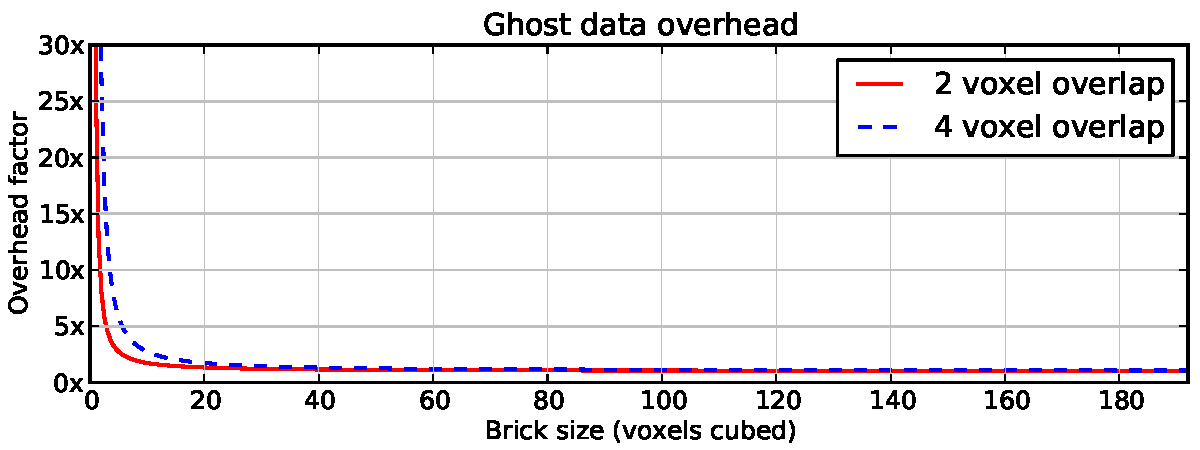
\includegraphics[width=0.99\linewidth]{images/rg/BS-overhead.pdf}
  \caption{Brick size overhead.  As bricks get smaller, the overhead
  for the additional ghost data grows significantly.  At a larger brick
  size of $128^3$, the overhead with 2 ghost voxels per dimension
  amounts to a few percent, whereas with $32^3$ bricks this increases
  the dataset size by almost 50\%.}
  \label{fig:brick-size}
\end{figure}

\subsection{Disk IO}

\subsubsection{Brick Layout}

Figure~\ref{fig:layout} demonstrates how this changes with the brick
size.  Both disk IO times as well as decompression times are displayed
there.  As shown in the figure, reading data from disk becomes quite
severe with small brick sizes.  However, as brick sizes grow to $64^3$
and beyond, decompression time becomes more important and overall time
plummets.  This effect is even more pronounced using a hard disk in
place of the SSD used here.  Intelligent layout strategies purport to
minimize seek times; our results corroborate this, with the important
caveat that seek times are not relevant with larger brick sizes.

\begin{figure}[tb]
  \centering
  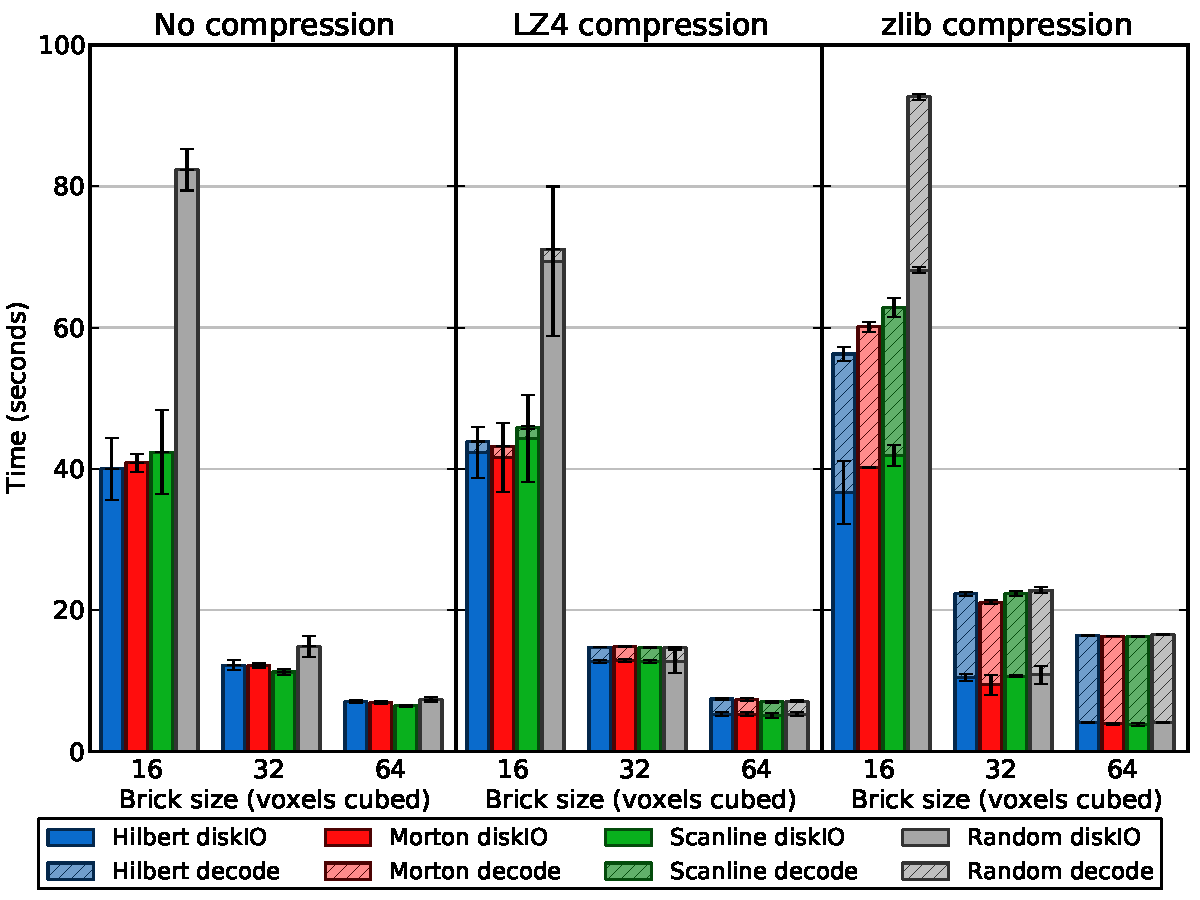
\includegraphics[width=1.00\linewidth]{images/rg/brickIO-RichtmyerMeshkov-ZoomIn-SSD.pdf}

  \caption{Time spent with IO-related tasks using an SSD for the
  RMI dataset's zoom-in scenario, sampled with 100 frames and a
  $1024\times768$ viewport.  Layout strategies only see utility at
  small brick sizes.}

  \label{fig:layout}
\end{figure}

% \begin{figure}
%   \centering
%   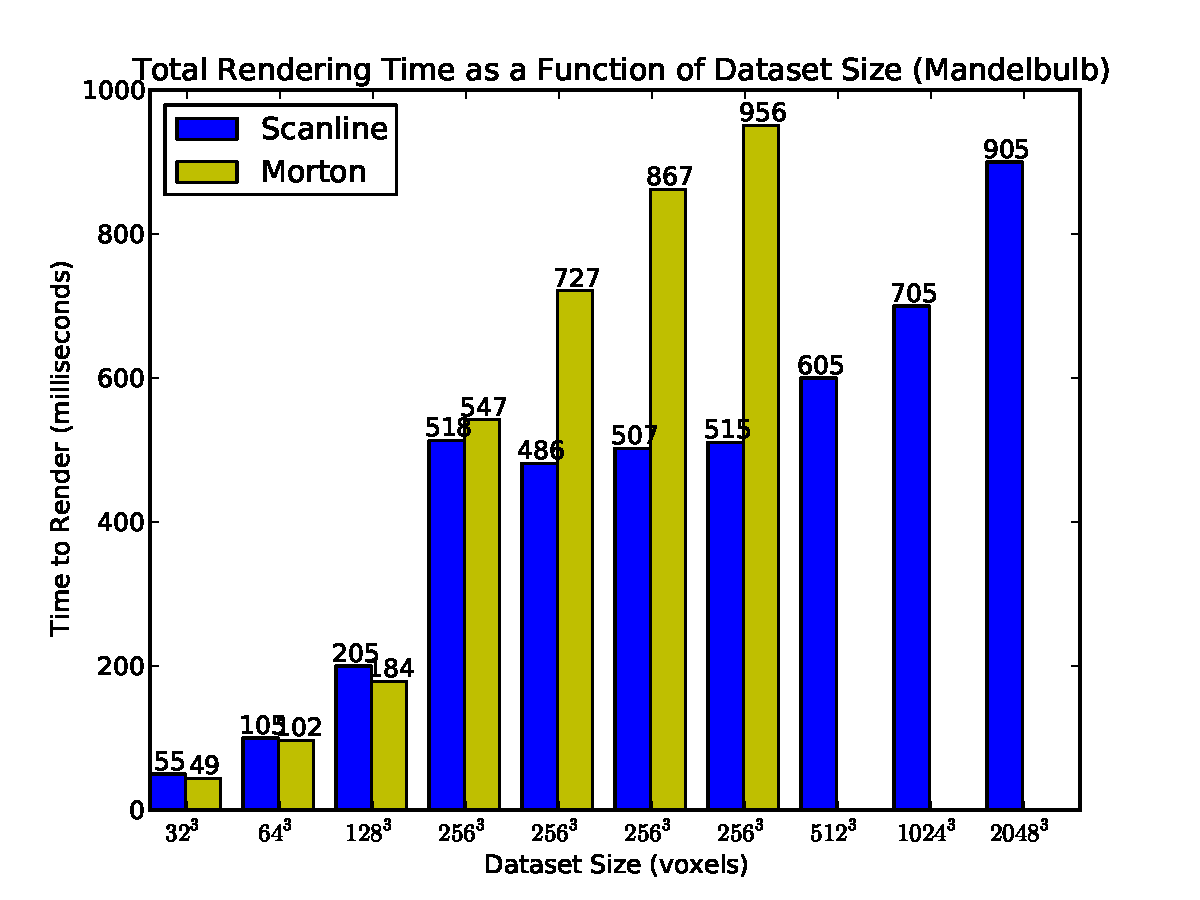
\includegraphics[width=\linewidth]{images/dsize-rtime}
%   \caption{\todo{needs update, data is made up (alex: benchmark! run
%   dsize-performance.lua)} Total rendering time, including brick IO,
%   to generate animations for the `mandelbulb' dataset at various
%   sizes and two distinct layouts.  Brick size was $32^3$ for all
%   runs.  Layout scheme has relatively little impact: disk read time is
%   negligible relative to the entire process.}
%   \label{fig:rtime-layout}
% \end{figure}

\subsubsection{Dynamic Rebricking}
\label{sec:rebricking}

% \todo{this is too long. important message: rebricking is a good idea,
% because it avoids absurd hierarchy build times and gives good I/O
% performance. the overhead is demonstrably minor.}

The renderer desires small bricks, as discussed in
Section~\ref{sec:subdivision}, as small bricks will help with early ray
termination and empty space leaping.  However Figures~\ref{fig:layout}
and \ref{fig:brick-size} clearly demonstrate that large brick sizes
are preferable for disk performance and overhead reasons.  To provide
the best of both worlds, we implemented a `dynamic' bricking scheme,
whereby bricks are stored on disk in a rather large size (e.g. $256^3$)
but presented to the renderer as if they exist at some small resolution
($32^3$).  The small bricks are dynamically generated from the large ones on
request.

Since requesting a large brick for every small brick would only
increase the disk traffic, we keep an additional brick cache in memory
to source these copies from.  Our cache uses a standard LRU strategy.
This is advantageous when the working set of the data fits into the
host memory, however when the working set exceeds the host memory we
will evict entries before finishing a rendering.  We stuck with this
strategy since the working set
often \emph{does} fit into host memory, as established by
Figure~\ref{fig:working-set}.  If the renderer is to be used in an
environment in which working sets are routinely larger than memory, an
MRU strategy would be more appropriate.

\paragraph{Hierarchy Generation}

Reorganizing data into a set of bricks is mostly ignored in volume
rendering literature, but becomes a significant bottleneck in
real-world usage.
Figure~\ref{fig:hierarchy-build} shows the time our preprocess needs
to generate this hierarchy, which increases sharply for small brick
sizes.  This time also increases with respect to dataset size.  At
the extreme scale, such data reorganization is completely infeasible:
merely reading every datum might take months.  We believe such
reorganization will be feasible up to a few tens of terabytes.  In
practice, the authors and collaborators thereof tolerate this for up to
4 terabytes at present.

% For the case of visualization-based verification, a dataset might
% only need to be loaded once to identify that a parameter was set
% wrong; this data reorganization is then a very high cost to pay.

Rebricking the data at run time alleviates this problem.  The data can
be generated at very large brick sizes, enabling fast conversion and
effective disk throughput, and then dynamically rebricked to very small
sizes.  Both disk and renderer deal with their ideal cases, then.  The
`Rebricking' case of Figure~\ref{fig:breakdown} shows performance in
this mode.

%% compression isn't unique enough to have its own story, particularly
%% since we need space.

% \subsubsection{Compression}
% 
% Regular gridded data typically contains large areas of uniform
% values.  One example is in the outer regions: most scanners as well as
% simulation software produce many layers of zeroes outside the region of
% interest.  Especially in simulation output, there may be large areas in
% a dataset which change at a very low frequency, producing runs of the
% same data value. All of these regions compress very effectively.
% 
% \todo{make it clear we are compressing each brick in isolation, storing
% it compressed on disk, and decompressing it when it is read---before it
% makes it to the renderer}
%
% \begin{figure}
%   \centering
%   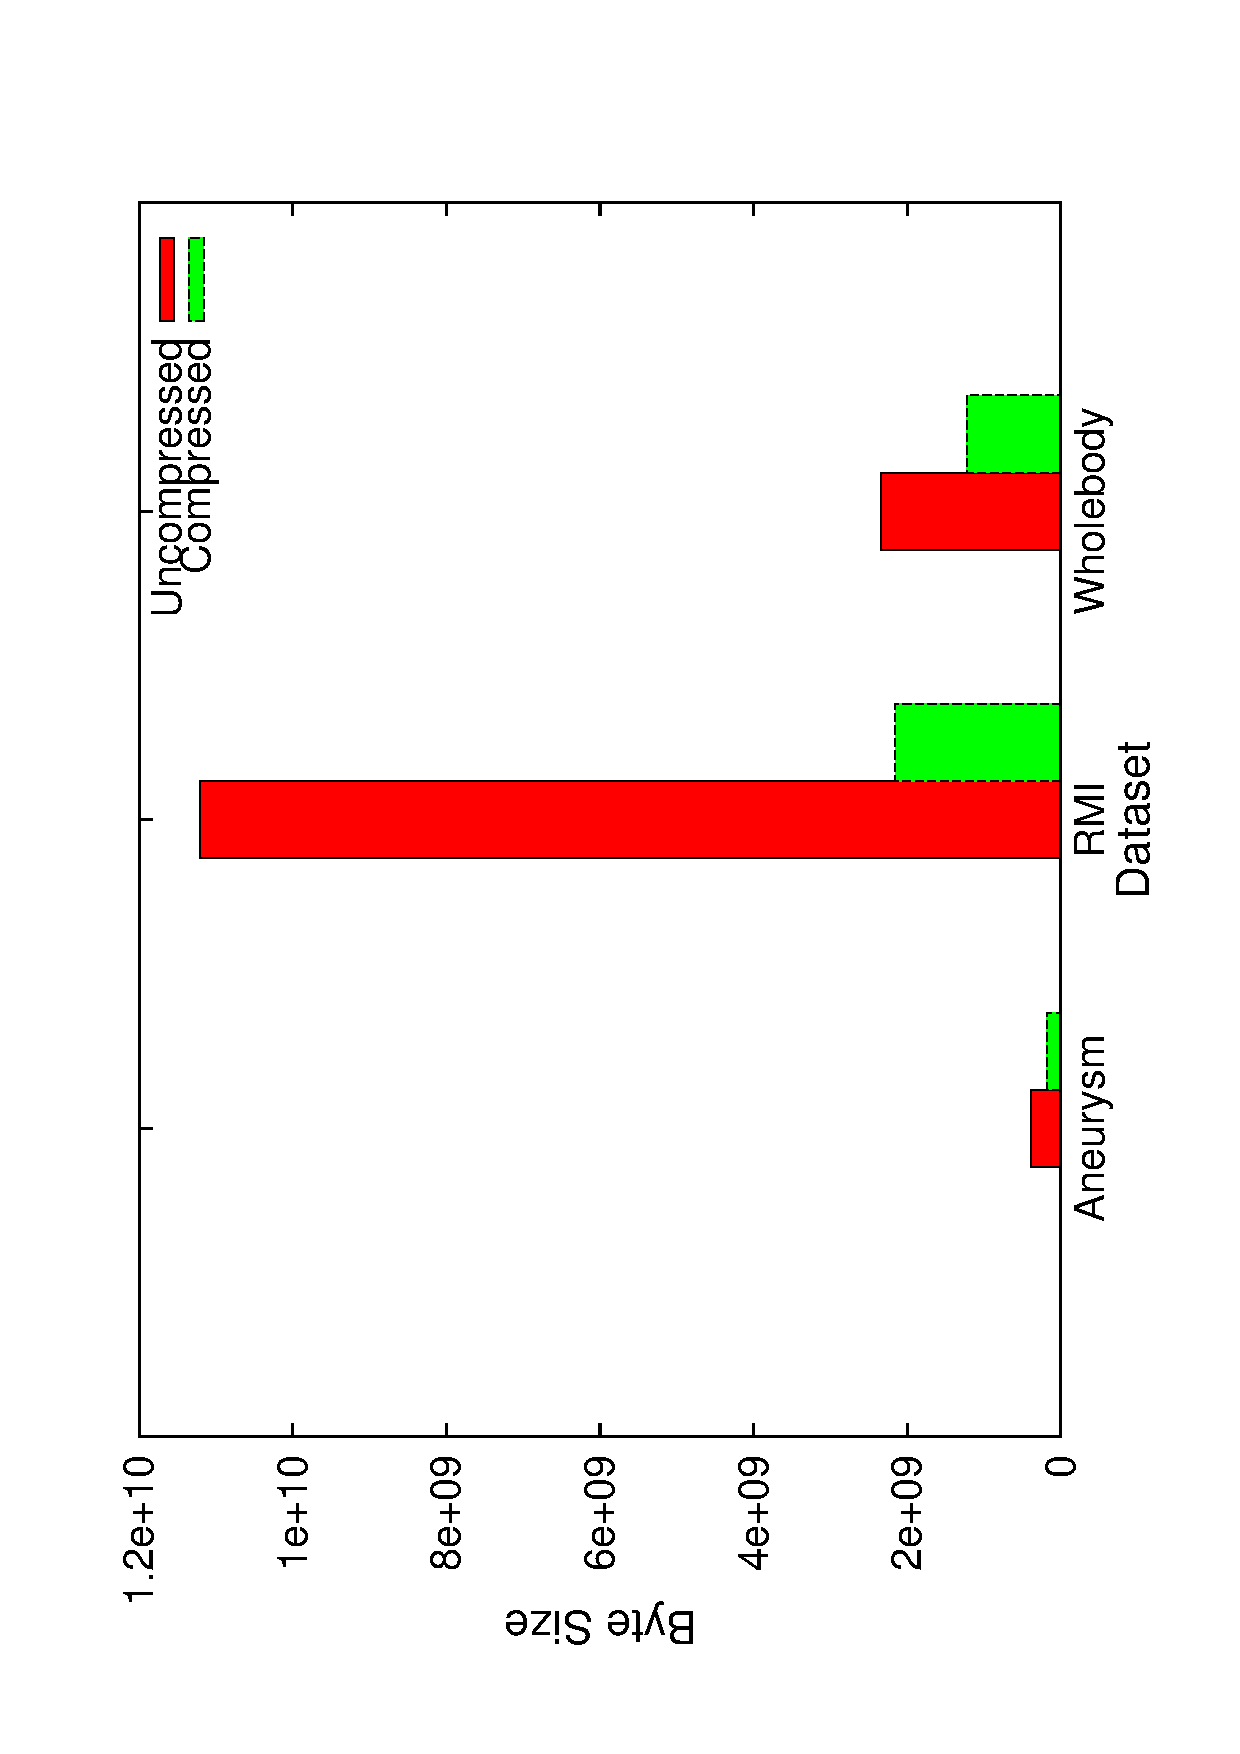
\includegraphics[width=\linewidth]{images/Compression}
%   \caption{Compression ratios for a variety of datasets using the
%   `fastest' zlib compression mode.  Very often, data compress to a
%   factor of less than half their original size. \todo{Alex will replace
%   this graph}}
%   \label{fig:compression}
% \end{figure}
%
% \todo{Need results for (\emph{many}!) more datasets!}

% The zlib libary has given us very good results for many datasets.
% Some results on the compression ratio are given in Figure
% \ref{fig:compression}.  Our system compresses data per-brick, and is
% instrumented to keep track of the data sizes both before and after
% compression.  Interestingly, these brick sizes \emph{always} shrink:
% we have not identified a single brick in any depicted (as well as many
% other) datasets for which the post-compression size is increased.  We
% attribute this to the addition of ghost data, which enlarges even the
% smallest brick to $3^3$.

\begin{figure}[tb]
  \centering
  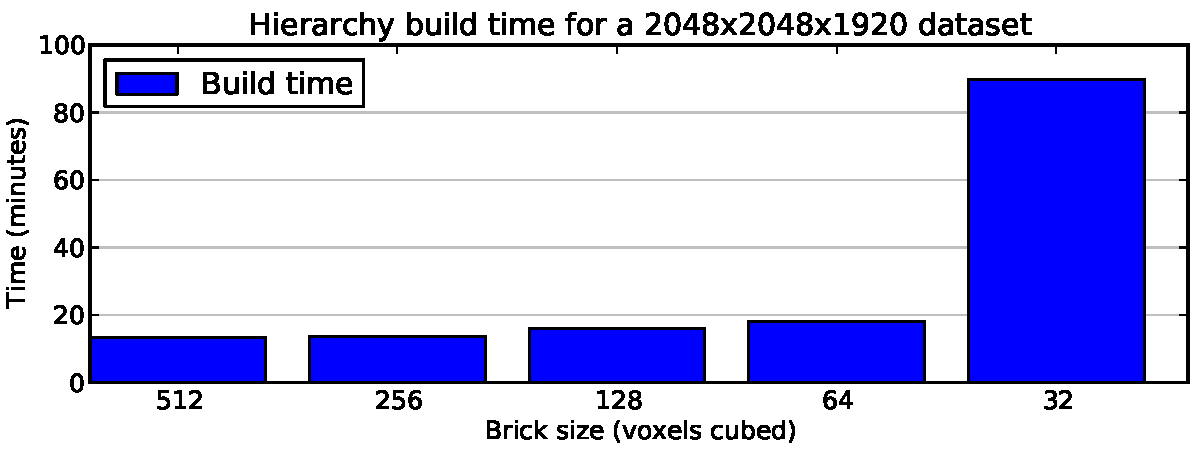
\includegraphics[width=0.98\linewidth]{images/rg/HierarchyBuildTime.pdf}
  \caption{Time to build bricked representation for a medium-sized dataset,
  as a function of brick size.  Renderers desire small bricks to
  perform efficiently, but generating such bricks takes significant
  preprocessing resources.}
  \label{fig:hierarchy-build}
\end{figure}


\begin{figure*}
  \centering
 \begin{minipage}[t]{0.3151225\linewidth}
   \begin{algorithm}[H]
   \caption{Greedy algorithm: request all bricks at all resolutions.}
     \begin{algorithmic}[H]
     \State ReportMissingBrick(\textit{b}) \Repeat
       \State \textit{LoD++}
       \State \textit{b} = LookupBrick(\textit{ray}, \textit{LoD})
       \If{Missing(\textit{b})}
         \State ReportMissingBrick($b$)
       \EndIf
     \Until{$\lnot$Missing(\textit{b})}\\
     \end{algorithmic}
   \end{algorithm}
 \end{minipage}
 \hfill
 \begin{minipage}[t]{0.65\linewidth}
   \begin{algorithm}[H]
   \caption{Global algorithm: only request bricks required to satisfy
   the final rendering request.\vspace{-0.185em}}
     \begin{algorithmic}[0]
       \State ReportMissingBrick(\textit{b})
       \Repeat
         \State \textit{LoD++}
         \State \textit{b} = LookupBrick(\textit{ray}, \textit{LoD})
       \Until{$\lnot$Missing(\textit{b})}
     \end{algorithmic}
     \vspace{1cm}
     \vspace{1.0700em}
   \end{algorithm}
 \end{minipage}

  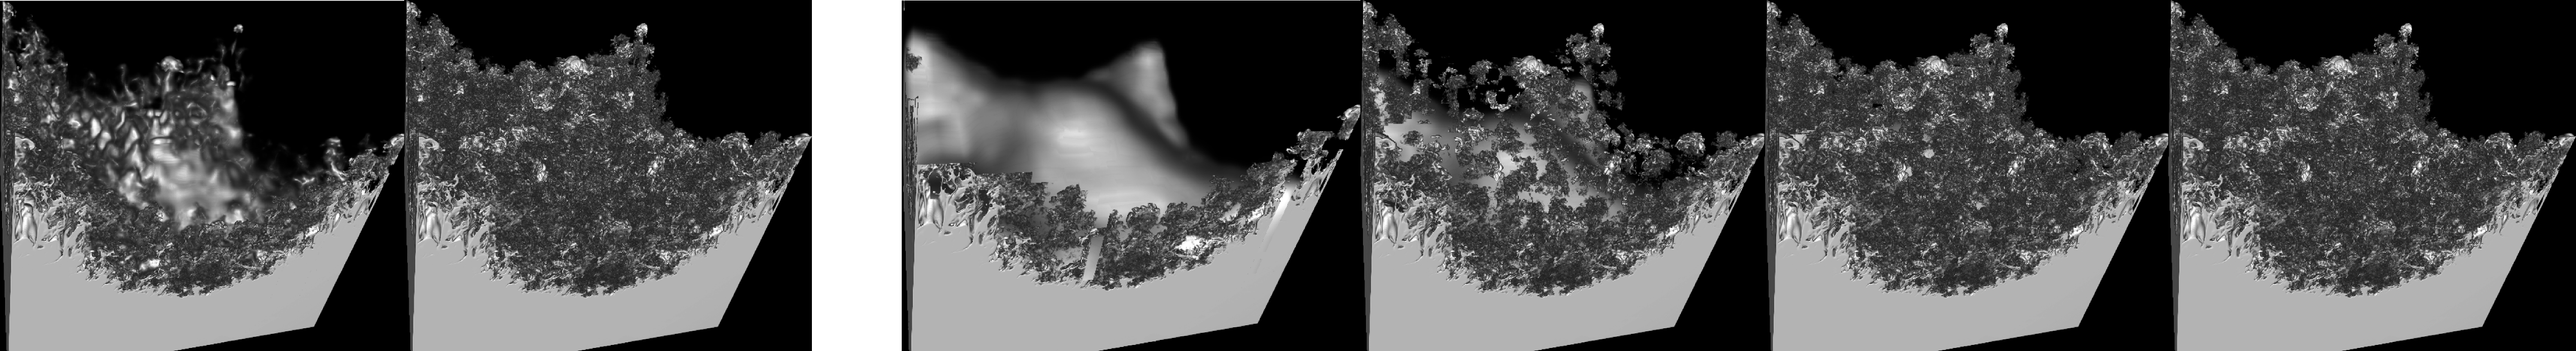
\includegraphics[width=\linewidth]{images/rg/strategy.png}
%   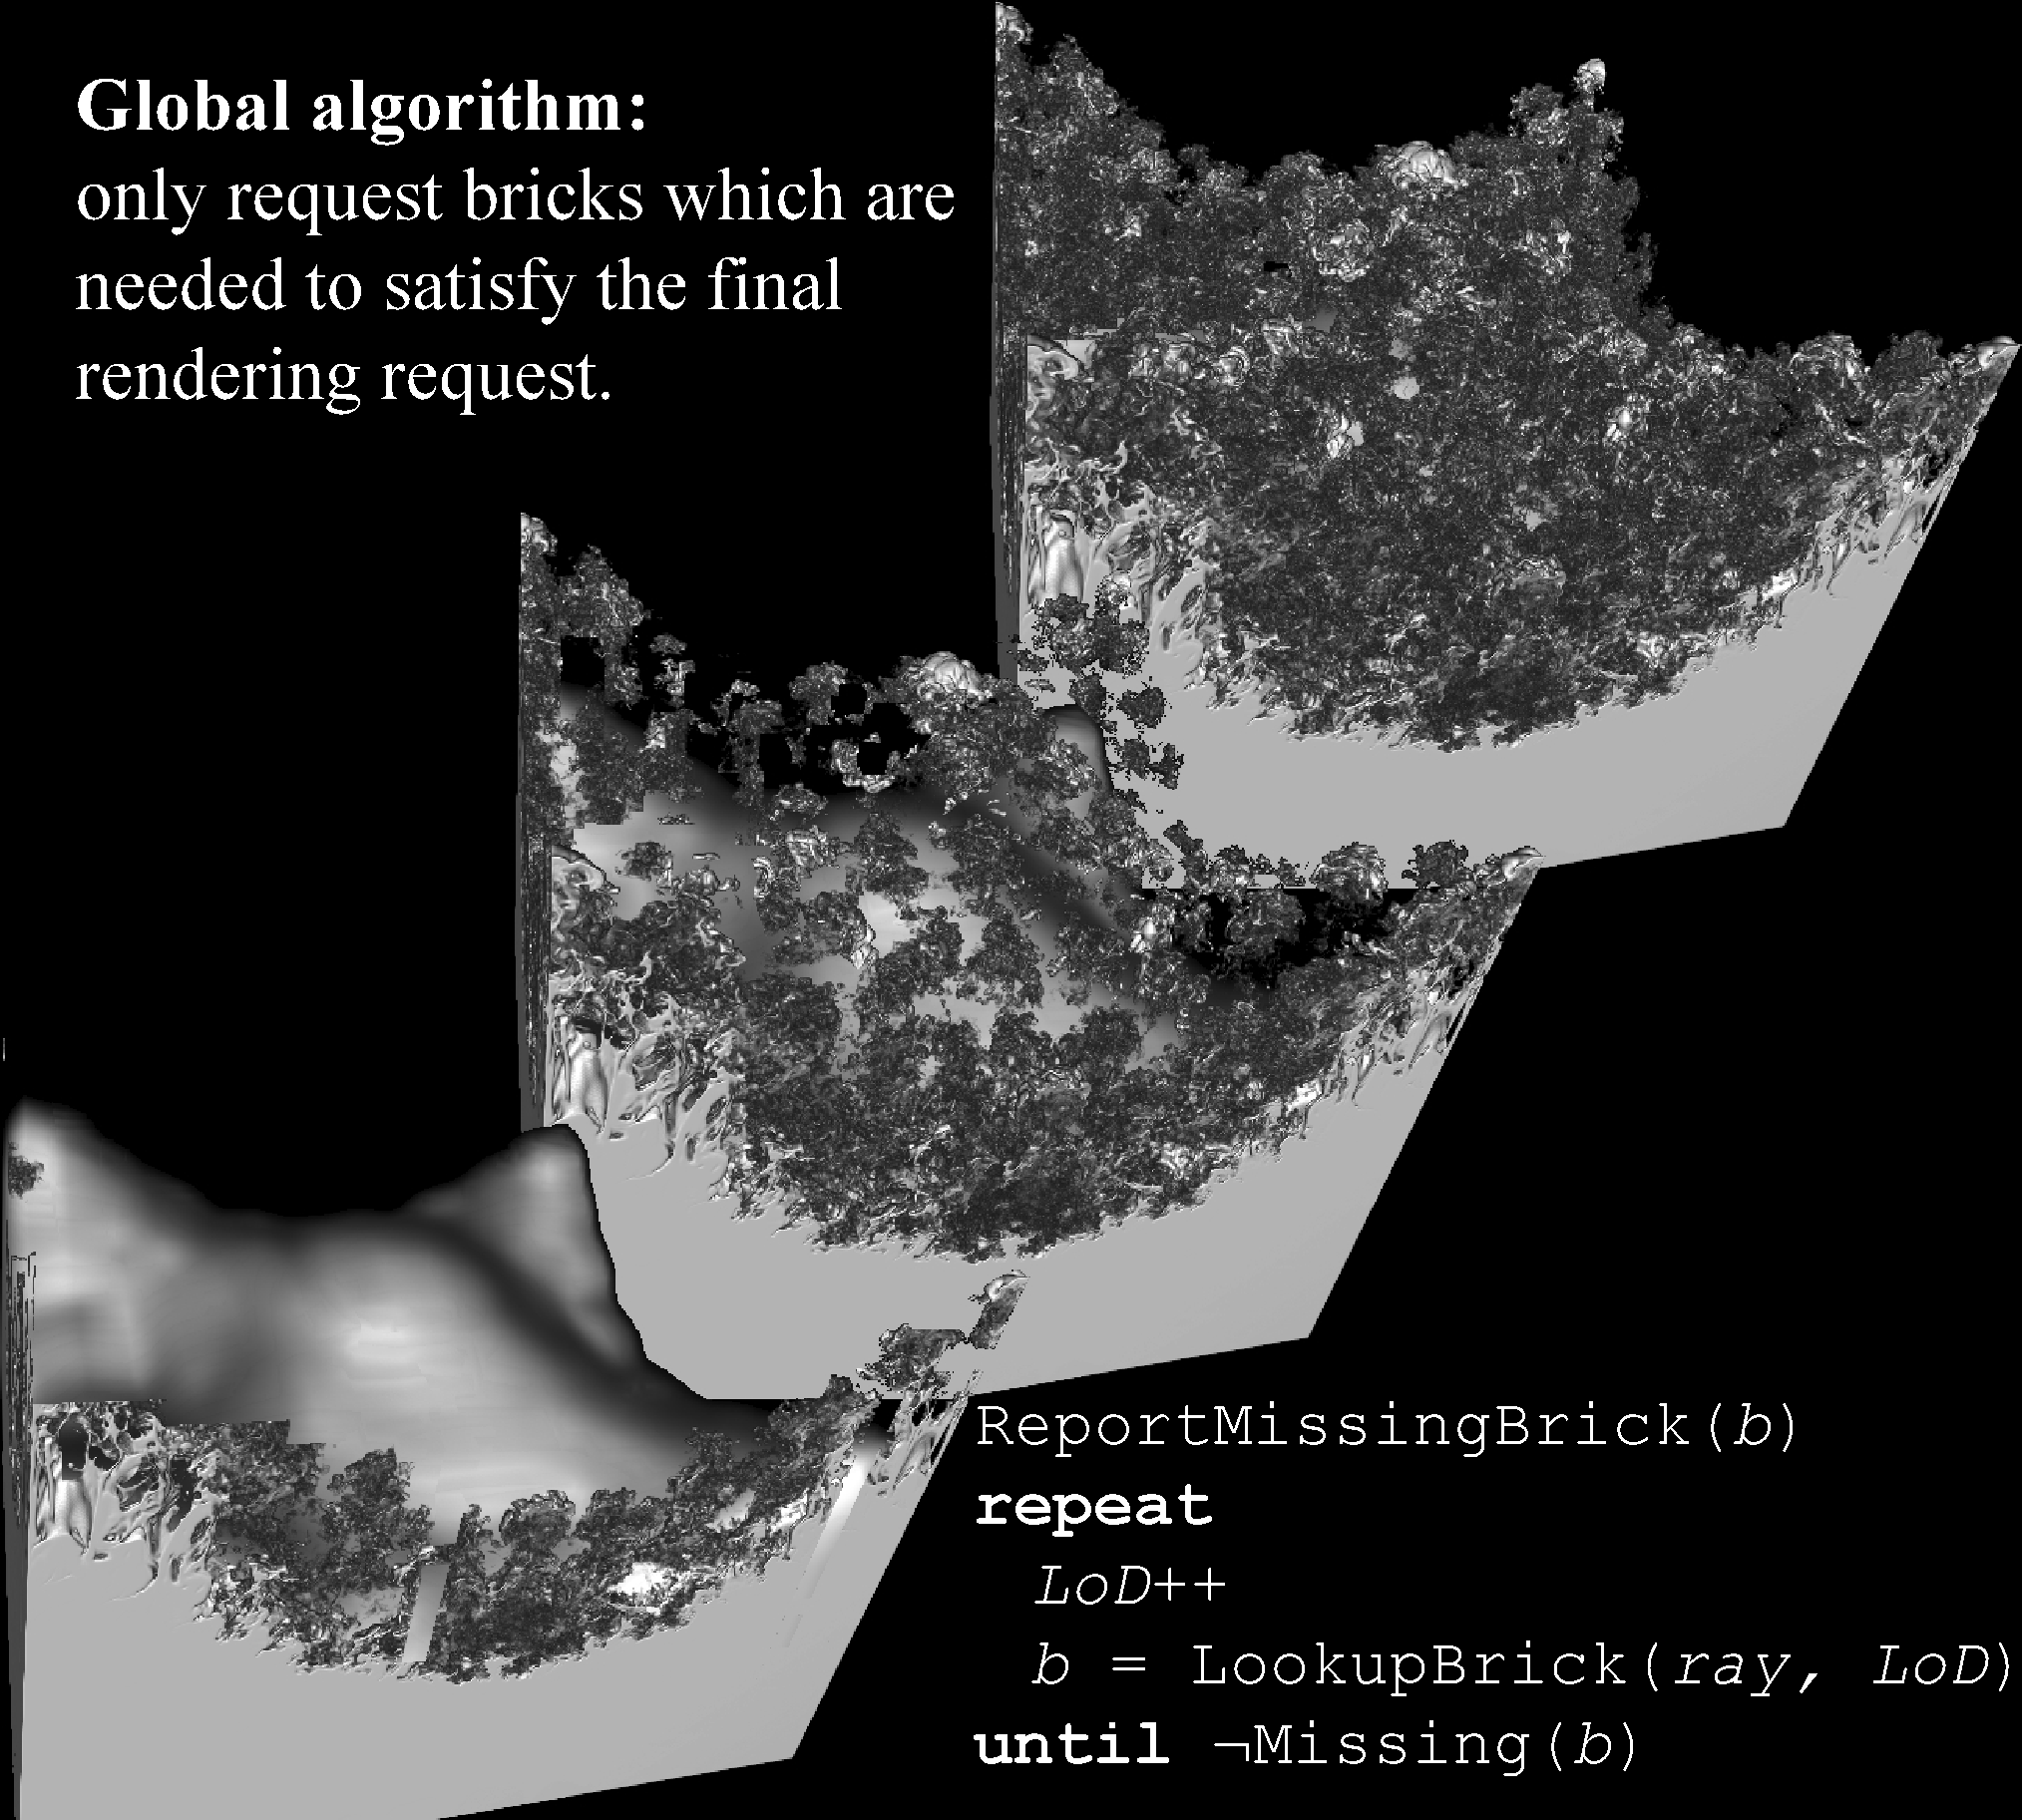
\includegraphics[width=0.99\linewidth]{images/Algorithm-Global}
%   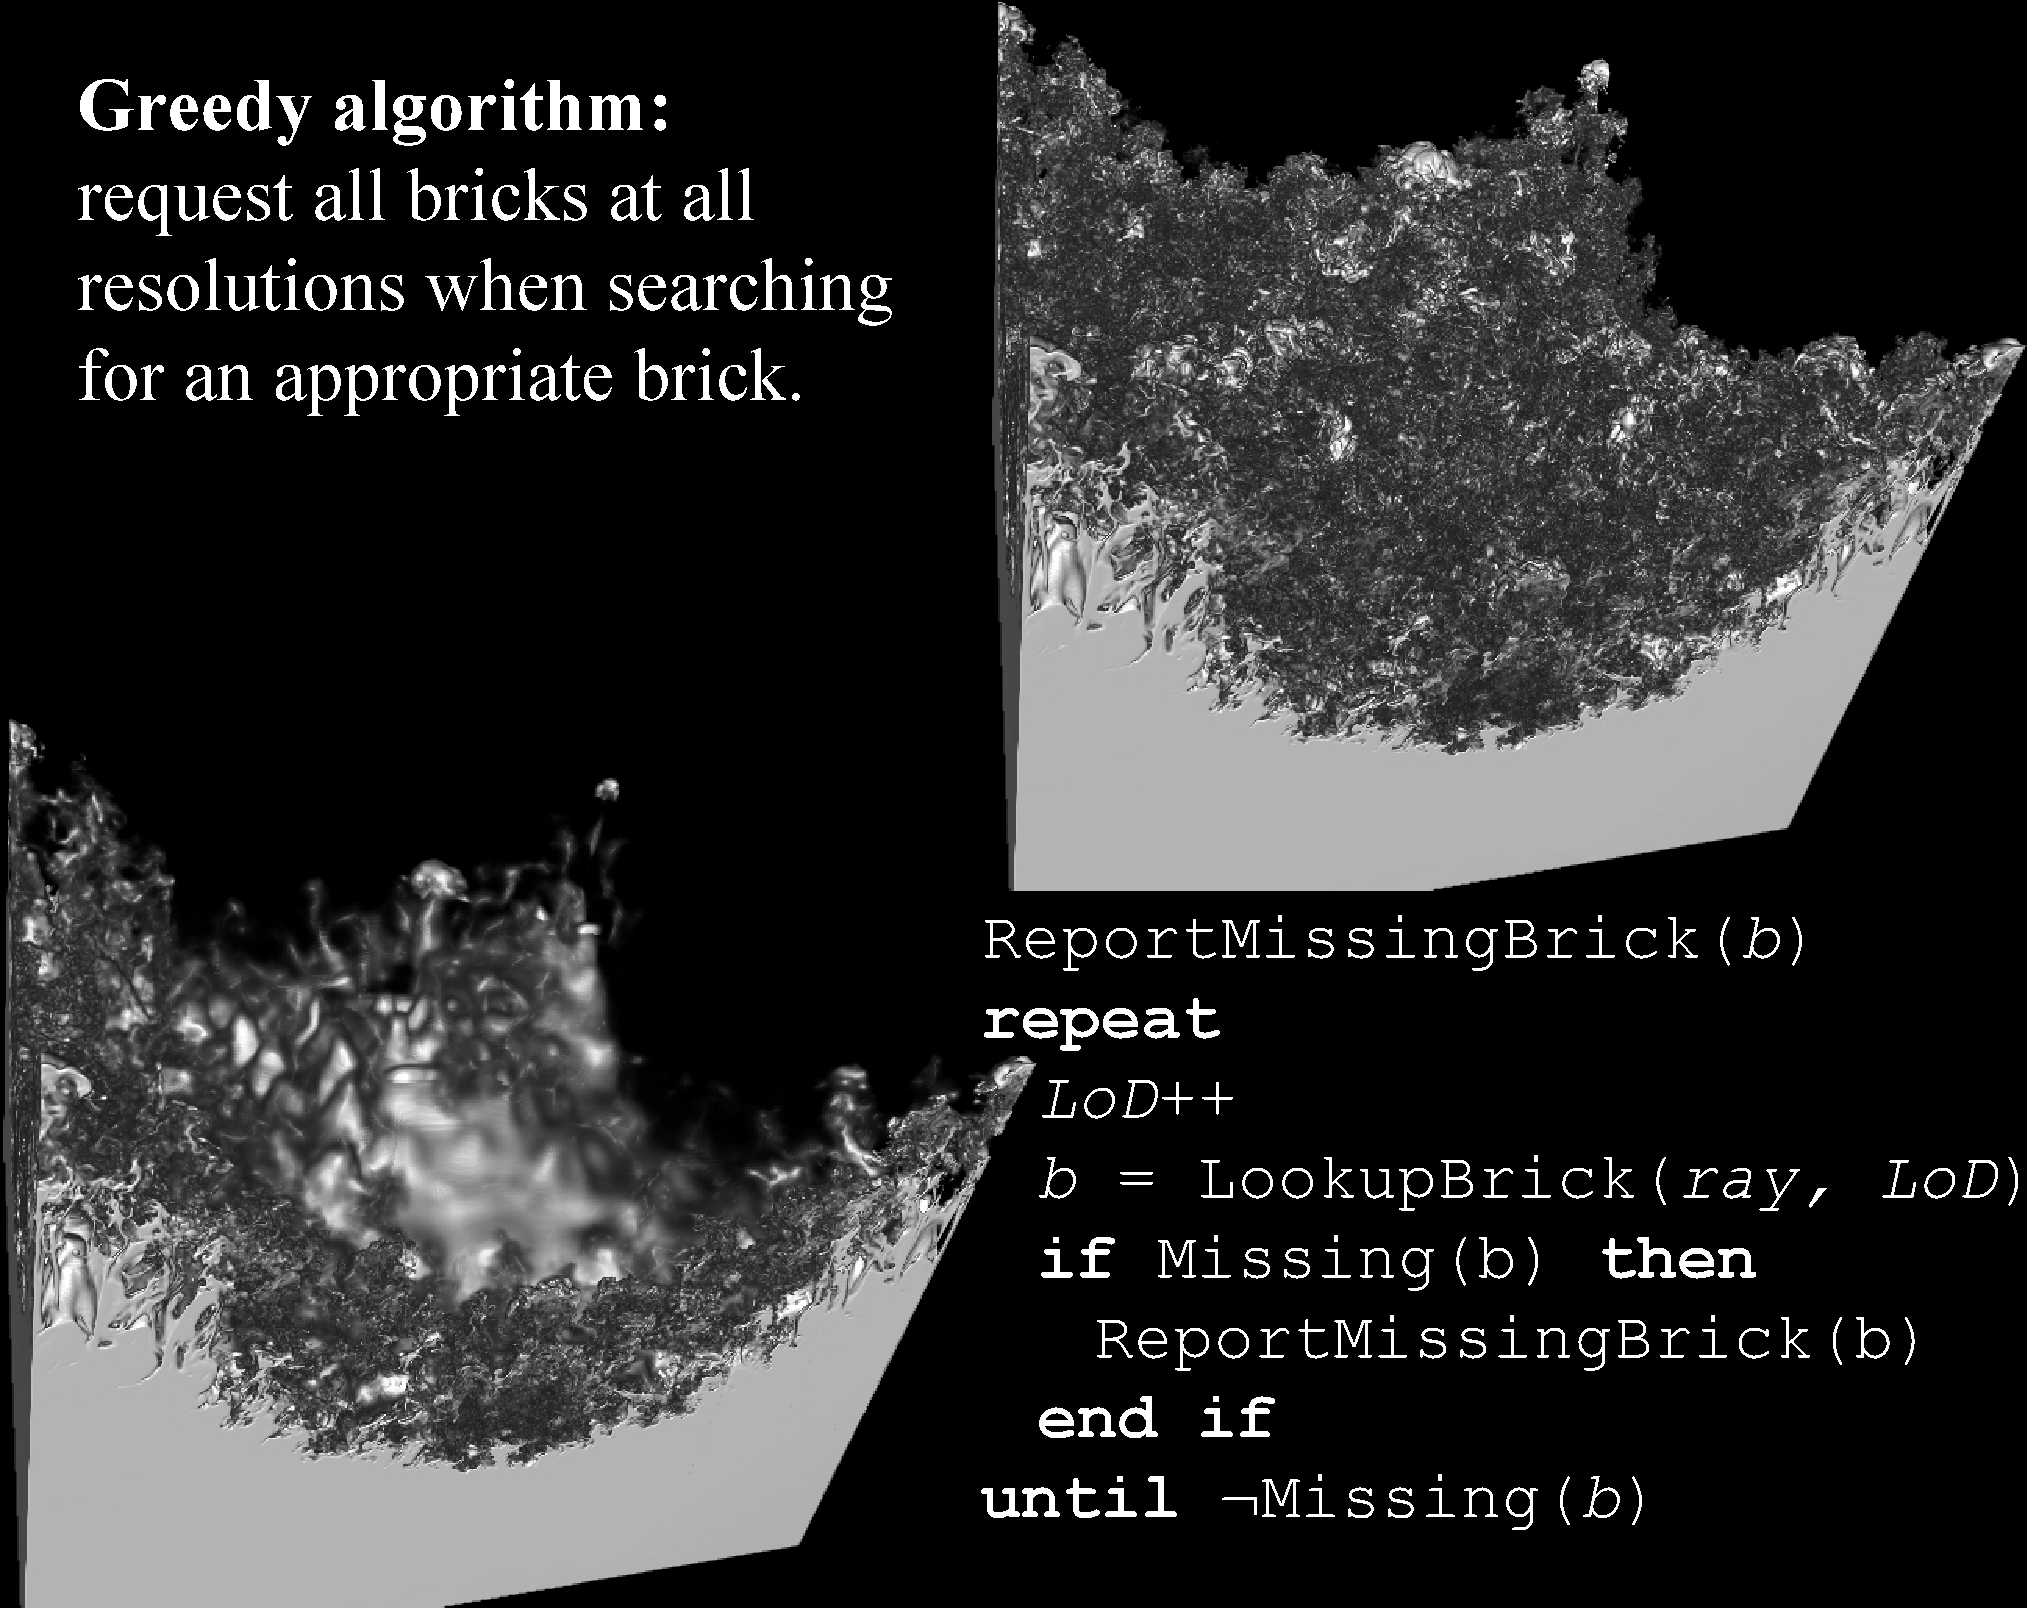
\includegraphics[width=0.99\linewidth]{images/Algorithm-Greedy}
  \caption{The effect of multiple brick replacement strategies.
  Renderings are select intermediate frames from the corresponding
  strategy.  `Greedy' strategies converge quicker and produce more
  densely-packed intermediate progress.}

  \label{fig:strategy}
\end{figure*}

\subsection{CPU/GPU Interface}

Point (4) in our overview is the efficient communication of the ray
guidance information from the location it is generated---the GPU---to
the location it is utilized---the IO layer of a volume renderer.  This
section details how that communication happens.

We utilize a GPU-based hash table to store this data, though we note
that we really only require a set.  That is, our keys (brick IDs) are
our values, and we only care about their \emph{presence} in the table,
which we will read back and process as a list later.  A list would work
as well, but a hashing scheme allows concurrent inserts to proceed with
less contention.  During rendering, a ray may write into this table to
indicate that it
needs a non-resident brick to continue (see Figure \ref{fig:flow},
(c)).  This small table will be read back from the GPU at the end of a
frame and utilized to fill the volume pool with new data.

As locks do not exist in current GLSL versions (and potentially never
will), lock-free structures are the only hazard-prone data structures
which can be correctly implemented.  Crassin et
al.\cite{Crassin:2009:Gigavoxels} workaround this by using multiple
render targets: each pixel has its own unique set of memory to
write into, and so there are no write hazards.  Our scheme requires
significantly less memory, but we must deal with these write hazards.

\subsubsection{Hash Table Parameters}
\label{sec:ht-params}

We map from the 4D index of the requested brick (spatial index + LoD)
to a unique 1D index in the hash table.  The mapping we utilize is
simply converting the 4D index into its equivalent 1D form, as if it
were stored in a 1D array.  We increment the index by 1 so that we may
use 0 to indicate that there is no entry at a location.

In a normal concurrent hash table, a lock is acquired for a table or
bucket before an access.  In lock-free data structures the primitives
used to implement locks are instead used directly on the data values
in question.  Inserts into our table proceed mostly as described in
previous
work~\cite{Michael:2002:LockFreeHT}.  In the face of concurrent
writes, this operation fails, and we attempt to probe a few times
(presently: 10) before giving up.

The critical piece to note is: \emph{it is not an error if a
missing brick is not recorded}.  As long as \emph{some}
missing bricks are recorded, the next frame \emph{will} make progress.
Each ray is either: finished, able to make progress, or unable to make
progress due to a lack of bricks that it requires.  Since our hash
table only contains entries for bricks which were requested by a ray,
then an invariant of our system is that: volume rendering is done, or
there exists at least one ray which can make progress.

% When a large number of bricks are needed, the hash table fills
% consistently, implying that collisions are infrequent or unimportant.
% If we vary the number of times rehashing is attempted from 5 to 100,
% for example, then performance differs by less than sampling noise,
% and the number of subframes decreases by barely 5\%, suggesting that
% collisions happen infrequently.

% Intuitively, the hash table size would have a large effect on
% performance.  Large tables should enable recording \emph{every}
% missing brick in a single pass, reducing the number of total passes
% required before convergence.  However, we found the size parameter
% to be negligible.  Regardless of how many rendering passes one does,
% the overall work is the same: the number of rendering passes will not
% change the number of bricks which must be loaded and rendered.  The
% only additional cost to an extra pass is the per-frame setup, which
% is independent of data size.
%
% One effect that small hash tables \emph{do} have is that they improve
% the response time of the renderer.  Since the next frame cannot begin
% until all bricks in the hash table are loaded, a small hash table
% creates a more iterative, progressive rendering experience.

\subsubsection{Strategies for Loading Coarser Bricks}

When the resolution required is missing during ray-casting, a ray's
brick requests can be what we call `greedy' or `global'.  In the
`greedy' case, the ray requests intermediate levels of detail along the
way, flooding the hash table with
requests that \textit{this} ray wants.  In the `global' case, each
ray only requests what it absolutely needs, leaving space for other
rays to request what they need.  These cases are visually depicted and
expounded in Figure
\ref{fig:strategy}.

% \begin{figure}
%   \centering
%   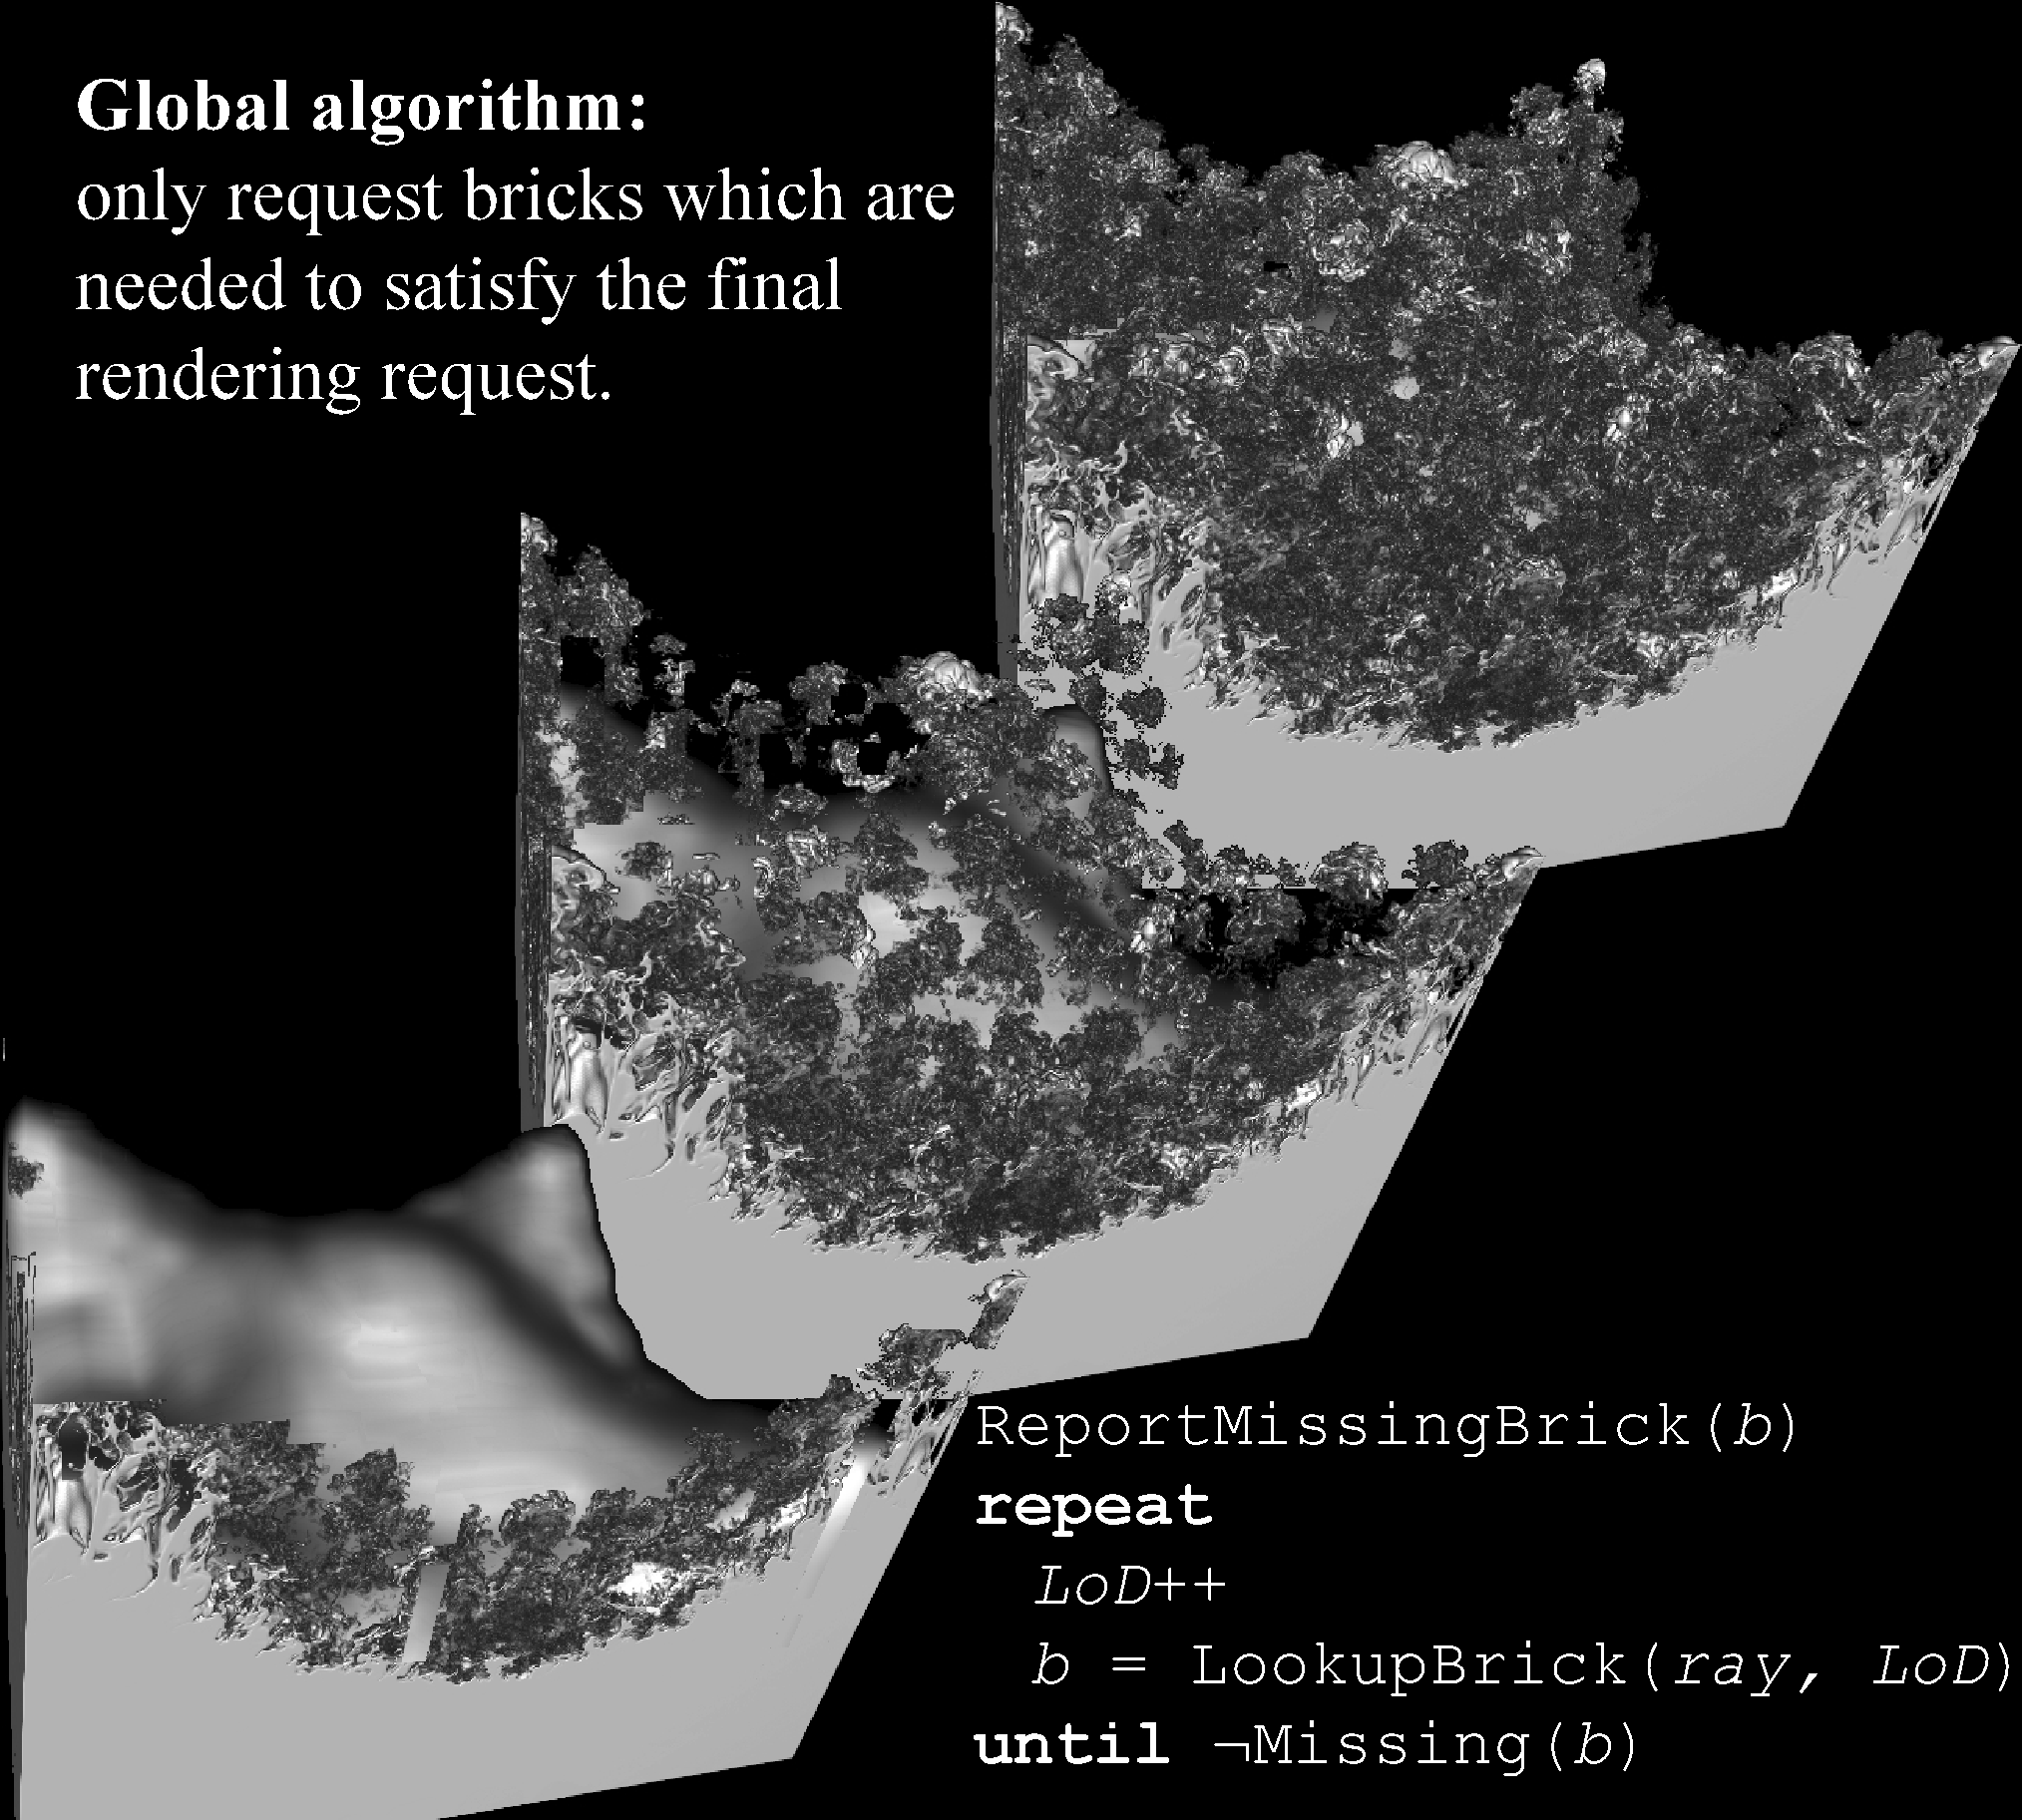
\includegraphics[width=0.99\linewidth]{images/Algorithm-Global}
%   \caption{The effect of multiple brick replacement strategies.
%   Renderings are select intermediate frames from the corresponding
%   strategy.  `Greedy' strategies converge quicker and produce more
%   densely-packed intermediate progress.}

%   \label{fig:strategyGlobal}
% \end{figure}

% \begin{figure}
%   \centering
%   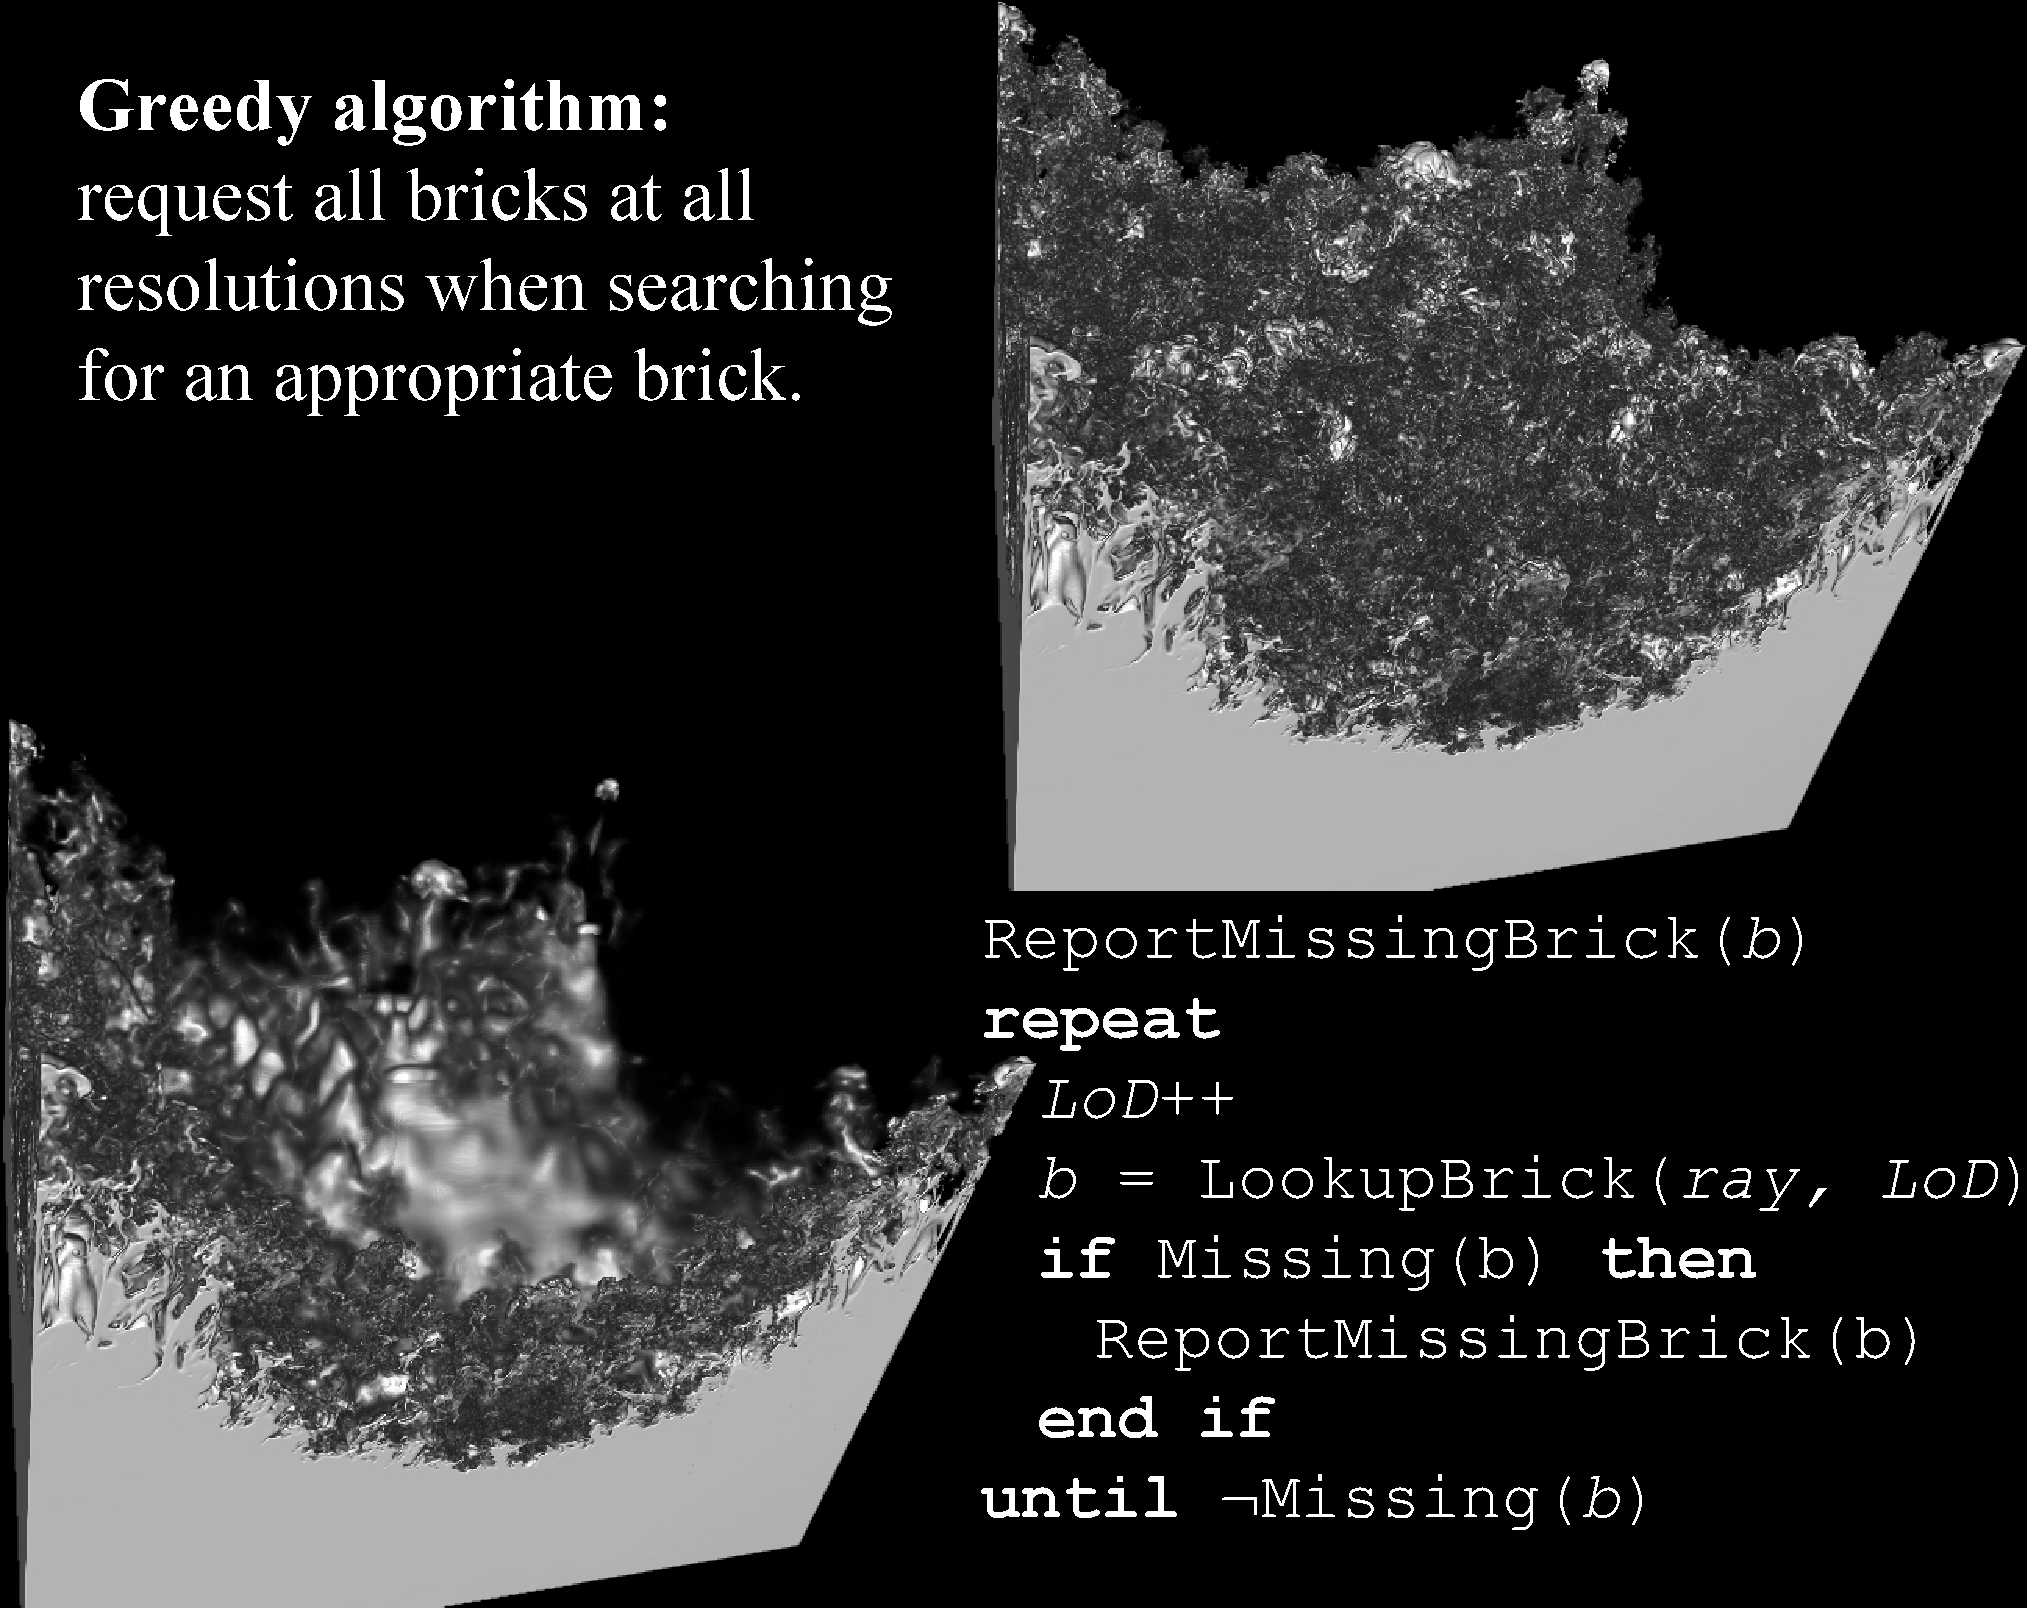
\includegraphics[width=0.99\linewidth]{images/Algorithm-Greedy}
%   \caption{The effect of multiple brick replacement strategies.
%   Renderings are select intermediate frames from the corresponding
%   strategy.  `Greedy' strategies converge quicker and produce more
%   densely-packed intermediate progress.}

%   \label{fig:strategyGreedy}
% \end{figure}

The intuitive interpretation is that the `greedy' approach will produce
a more responsive, iteratively-refined image, whereas the `global'
approach will generate the final correct image quickest.  However, the
authors were surprised to find that the `greedy' approach both produces
more pleasing progress information \emph{and} converges in the fewest
number of frames.  This is because it allows a ray to sample at its
final resolution quickly, which can cause earlier ray termination.

\section{Conclusions, Limitations, \& Future Work}
\label{sec:conclusion}

In this work, we have introduced an efficient, out-of-core, ray guided
GPU volume renderer which scales to extremely large data.  The system
pulls inspiration from a patchwork of recent renderers, combining the
advantages of many and reimplementing some ideas in light of modern GPU
features.  We have also contributed an evaluation and discussion of the
tradeoffs inherent in the development of a modern ray-guided volume
renderer.

Based on the data here, we conclude that a ray-guided volume renderer
should work with bricks which are, on disk, $64^3$ or larger.  This
minimizes time spent doing IO (Figure~\ref{fig:layout}), and makes
data layout irrelevant, obviating the need for a complicated component
of the code.  Since the required memory shrinks with the brick size,
generating $32^3$ or even $16^3$ bricks on-the-fly is desirable, though
which size is unfortunately too data-specific to answer generally.
While `bzlib' gives ideal compression ratios, it is very slow to
decompress, and therefore most implementations will want to utilize
`LZ4' compression.  A cache is a boon when data will not fit in GPU
memory but will fit in the host's memory.

We have made a best-effort attempt to design both favorable and
unfavorable conditions with which to test a volume renderer, but it
is possible some considerations have been omitted.  In particular,
this renderer and many others rely heavily on the assumption that
rays will saturate quickly.  Subjectively, we have found this to be
overwhelmingly valid for all our work in volume rendering, but this is
not a rule and has not been thoroughly evaluated.

A second issue is the rendering modes evaluated.  While our system
supports 2D transfer functions as well, all performance results
presented here utilized the 1D transfer function mode.  Advanced
rendering effects as well, such as those similar to ambient
occlusion~\cite{Schott:2009:DAOVR}, are omitted.  Such effects should
have a variable impact, positively correlating to the proportion of
rendering vs. IO times presented in
Figure~\ref{fig:breakdown}.  Screen-space methods may provide
acceptable quality without (comparatively) impacting performance.

Finally, reformatting the data into a bricked hierarchy continues to
be the bane of high-performance volume rendering.  This result is not
expounded often enough in the literature.  We hope this paper helps
to reiterate to the community that the FLOPs may be free, but data
movement will kill performance.

More importantly, we have contributed an evaluation and discussion
of the issues inherent in the development of a ray guided volume
renderer. As has been demonstrated, many of these choices are not as
clear as previous reports may have inadvertently implied.  The results
presented in this work clearly depict the tradeoffs, to aid system
designers in creating volume renderers which suit their particular
environment.

We hope to extend this work to more diverse visualization scenarios.
Ray-guidance-based isosurface generation is a natural candidate for
these ideas.  Furthermore, a common use case is combining an isosurface
with volume rendering, which has the potential to significantly change
such aspects as the working set size.  The general idea that rendering
should drive the visualization pipeline---as opposed to passively
consuming the output of earlier operations---is one that is applicable
in a much wider sense than that presented here.

%\appendix
\section{Data and Performance Details}
\label{sec:data}

\begin{figure}
  \centering
  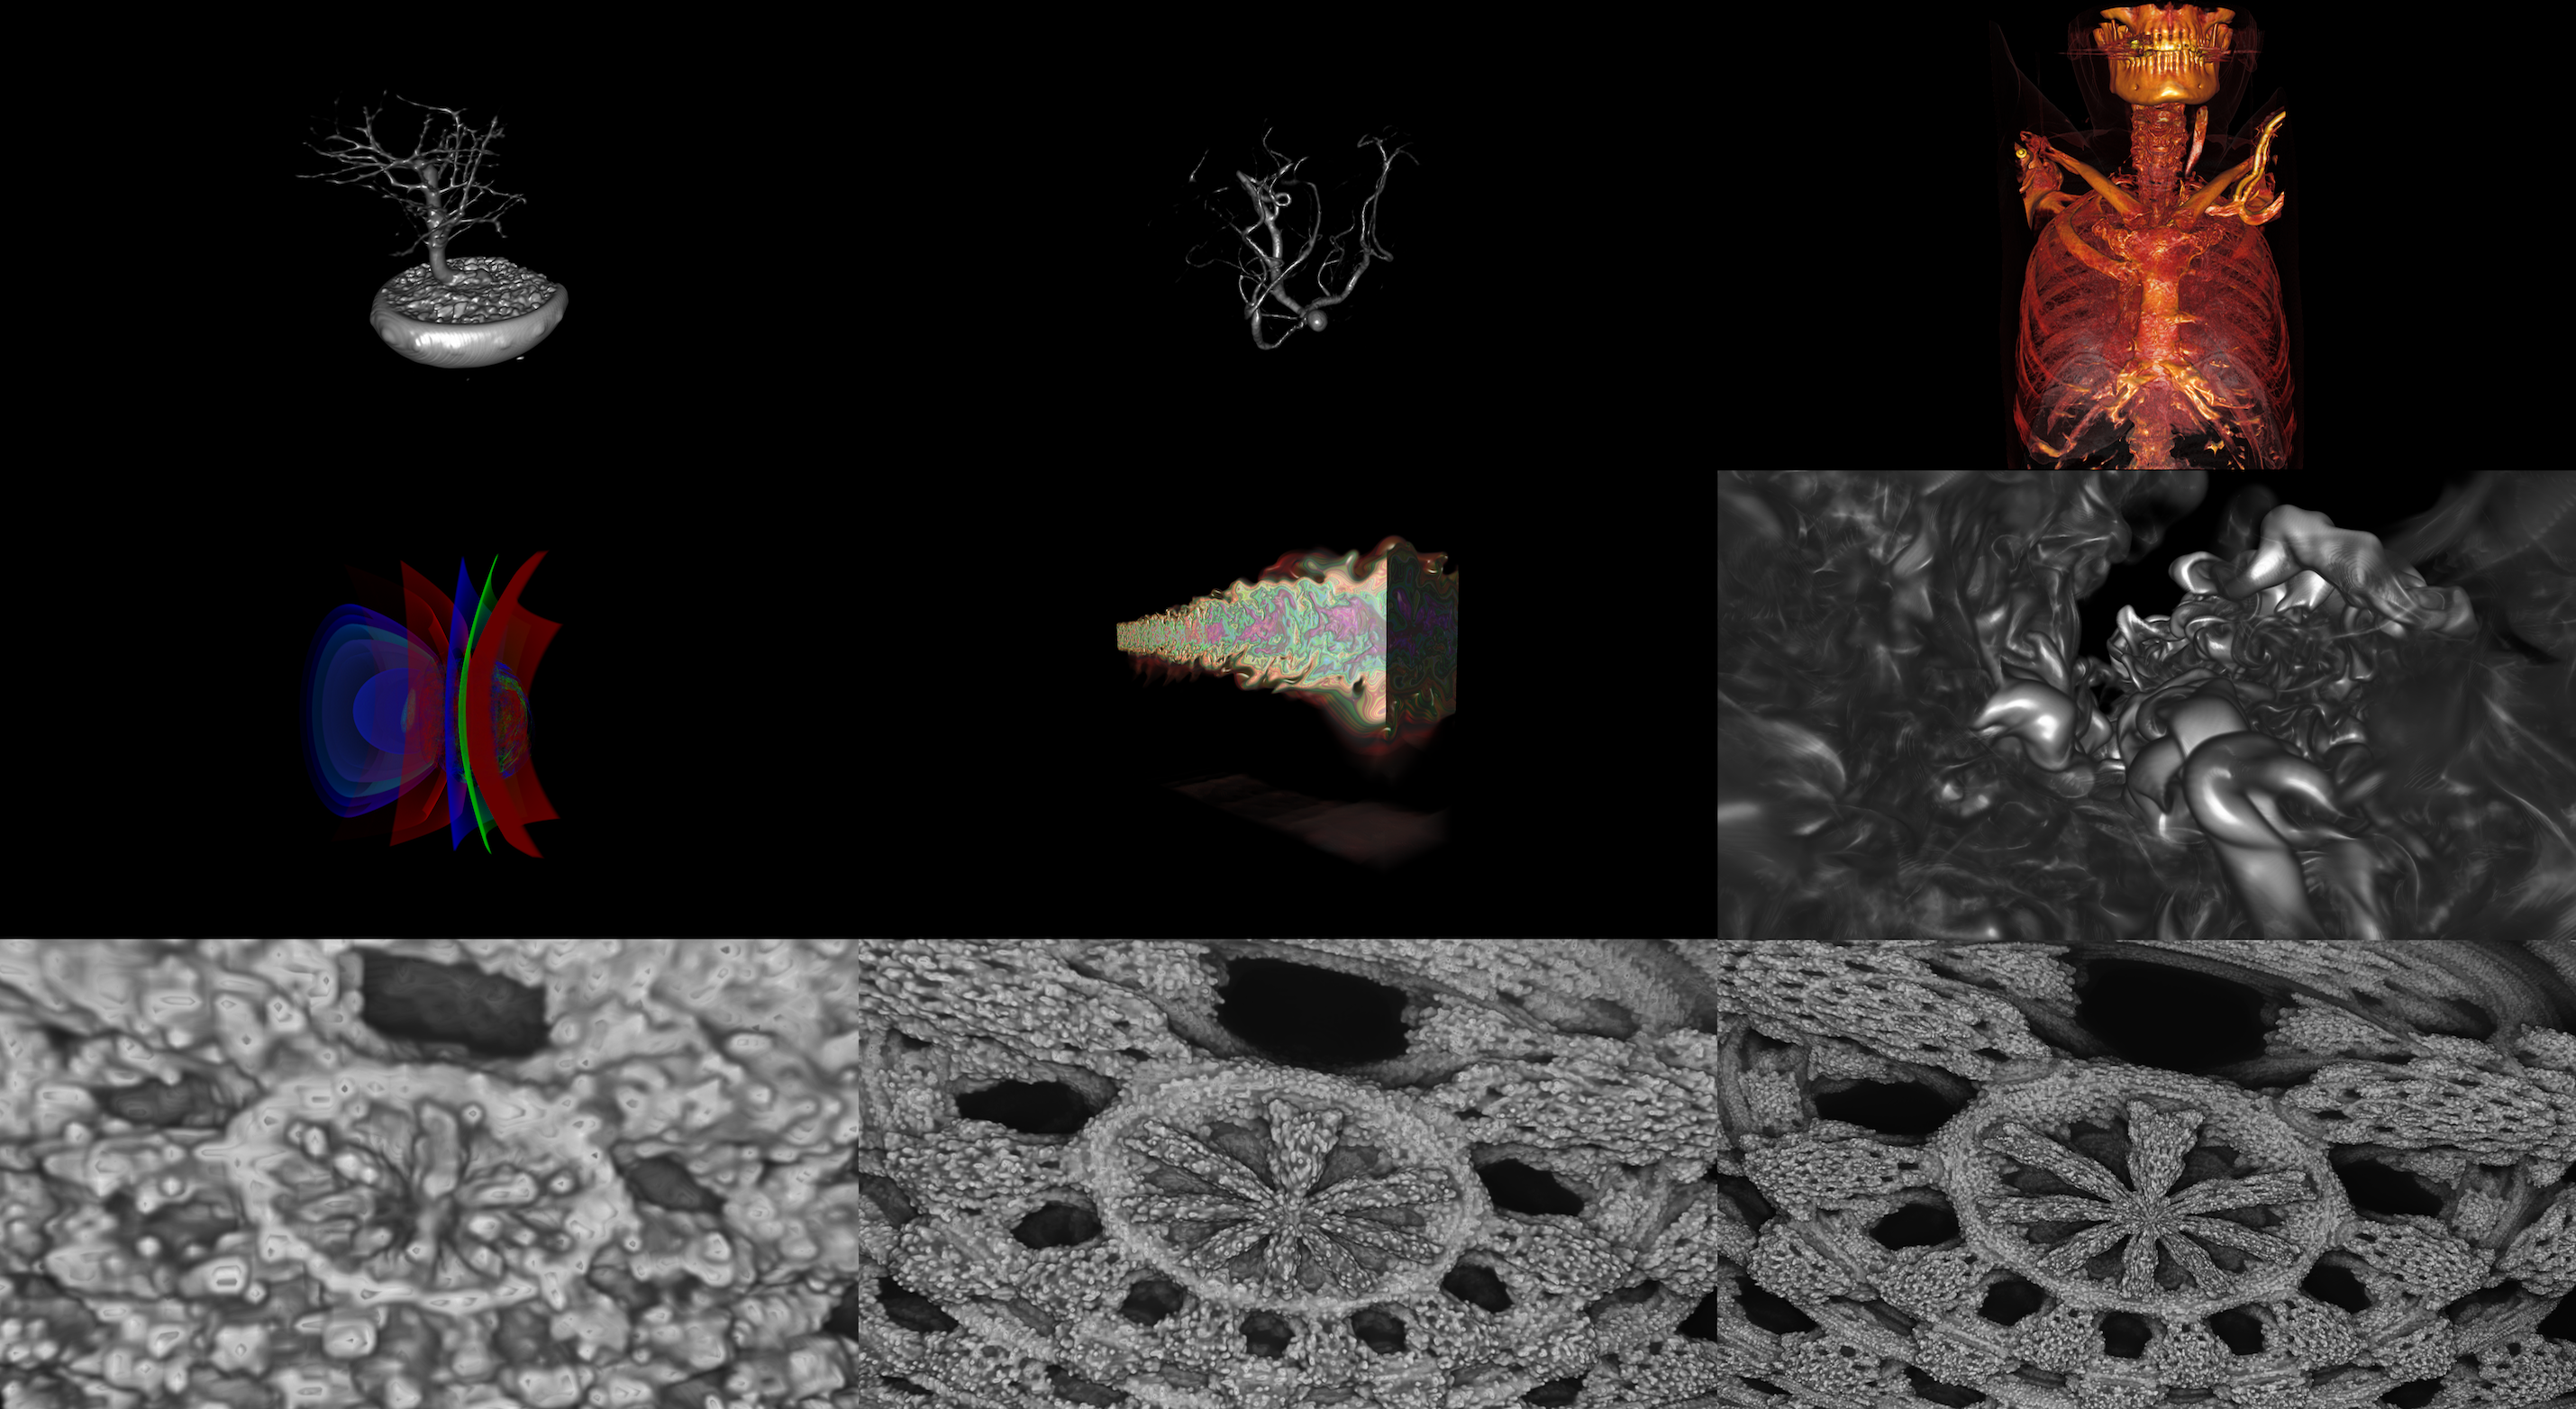
\includegraphics[width=0.98\linewidth]{images/rg/perFramesSmall.png}
  \caption{Selected frames from interactions used to record data for
  Table~\ref{tbl:timings} or Figure~\ref{fig:breakdown}}
  \label{fig:perFrames}
\end{figure}

We tested our renderer with a plethora of datasets, both real and
artificially created.  For space reasons, we discuss only a subset which
proved to be a reasonable sampling of our available data.
Renderer performance is depicted for a variety of datasets in
Table~\ref{tbl:timings}.  We discuss these in order of increasing size
here.

Two small datasets are the Bonsai tree (``Bonsai'') and ``Aneurysm''
datasets (Figure~\ref{fig:perFrames}, top, left \& middle). While
small by today's standards, effective empty space leaping and early ray
termination still double the performance
(Table~\ref{tbl:timings}, note how performance doubles with smaller
brick sizes).

The ``WholeBody'' dataset (Figure~\ref{fig:perFrames}, top, right) is
a contrast-enhanced CT scan of a human body.  As sometimes happens in
the biomedical domain, these data have limited slice resolution but a
plethora of slices.  Coarser resolutions must be careful to downsample
anisotropically, else the in-plane resolution washes out too quickly.

``Velocity'' (center, left) comes from the simulation of an exploding
star; we chose this dataset because our ideal transfer function for it
is quite transparent, preventing the renderer from taking advantage of
early ray termination.  Highly transparent transfer functions which
still produce informative results are a rarity but still occur.  For
these data, the additional overhead of small bricks can have a fairly
drastic effect on performance.  This dataset is one of the rare datasets
for which lighting actually makes the visualization more
\emph{difficult} to interpret, and so we always render this dataset
with lighting off.

The ``magnitude'' dataset (center, middle) comes from a combustion
simulation and represents another intermediate step towards larger
data.  The lower half of this dataset actually has a very faint trace
of data, which causes the renderer to sample densely.  The expense
of computing lighting information for fragments which ultimately
contribute very little has a notable effect on performance.

The Richtmyer-Meshkov Instability (``RMI'',
Figure~\ref{fig:teaser} right and Figure~\ref{fig:perFrames}, center,
right) and the Visible Human (Figure~\ref{fig:teaser} left) are popular
datasets in the volume rendering literature; details can be found in
previous work.

We created a series of ``Mandelbulbs'' at various resolutions ($1k^3$,
$4k^3$, $8k^3$).  These are an extension of the mandelbrot fractal into
3 dimensions.  This has many of the same properties of the data used in
Crassin et al.~\cite{Crassin:2009:Gigavoxels}, which took a large bone
scan and added Perlin noise to increase the sampling requirements.  We
create the high-resolution features \textit{a priori}, so no GPU
features were used to accelerate this process.  At equivalent
resolutions to that work, we see double to an order of magnitude
improved performance, but for this work we report results at 1080p HD
resolution.  A descriptive view of the Mandelbulb is
given in Figure~\ref{fig:bricks-empty} and there
are close-ups visible in Figure~\ref{fig:perFrames} (bottom row;
center, right).

\begin{table}
  \centering
  \caption{Per-frame rendering time at 6 different brick sizes, for
  a variety of datasets depicted in Figures~\ref{fig:perFrames} and
  \ref{fig:teaser}.  \textbf{Optimal brick sizes} are
  dataset dependent.}
  \label{tbl:timings}
  \rowcolors{4}{gray!20}{white}
  \begin{tabular*}{\linewidth}{|p{0.24\linewidth}|p{0.09\linewidth}|p{0.09\linewidth}|p{0.09\linewidth}|p{0.09\linewidth}|p{0.09\linewidth}|}\hline
    & \multicolumn{5}{c|}{\textbf{Rendering Time (ms)}}\\
    \cline{2-6}
    \multicolumn{1}{|l|}{\textbf{Dataset}}
                  & $16^3$ & $32^3$ & $64^3$ & $128^3$ & $256^3$ \\\hline
    Bonsai        & \textbf{16}     & 20     & 26      & 31      & 28     \\
    Head Aneurysm & \textbf{27}     & 34     & 40      & 55      & 85     \\
    Whole Body    & 140    & 94     & 82     & 77      & \textbf{67}      \\
    Velocity      & 376    & 208    & 146    & 118     & \textbf{110}     \\
    Magnitude     & 132    & 93     & \textbf{80}     & 82      & 85      \\
    RMI           & \textbf{60}     & 64     & 61     & 67      & 67      \\
    Visible Human & \textbf{34}     & 37     & 47     & 67      & 123     \\
    Mandelbulb1k  & \textbf{21}     & \textbf{21} & \textbf{21} & 22      & 25      \\
    Mandelbulb4k  & \textbf{27}     & 30     & 37     & 47      & 47      \\
    Mandelbulb8k  & \textbf{33}     & 37     & 45     & 60      & 78      \\\hline
  \end{tabular*}
\end{table}

\begin{table}
  \centering
  \caption{Dataset properties for test datasets.}
  \label{tbl:sizes}
  % color breaks the r@{sep} stuff.  great! <3 TeX.
  %\rowcolors{2}{gray!20}{white}
  \begin{tabular*}{\linewidth}{|p{0.24\linewidth}|p{0.085\linewidth}@{$\times$}p{0.085\linewidth}@{$\times$}p{0.085\linewidth}p{0.099\linewidth}@{\quad}|p{0.13\linewidth}|}\hline
    \multicolumn{1}{|l|}{\textbf{Dataset}} &
    \multicolumn{4}{c|}{\textbf{Resolution}} &
    \multicolumn{1}{c|}{\textbf{Size}}\\\hline
    Bonsai        & ~256 &$~256$ &$~256$ & 8 bpp  & 16 MB\\
    Head Aneurysm & ~512 &$~512$ &$~512$ & 16 bpp & 256 MB\\
    Whole Body    & ~512 &$~512$ &$3172$ & 16 bpp & 1.5 GB\\
    Velocity      & $1000$ &$1000$ &$1000$ & 16 bpp & 1.9 GB\\
    Magnitude     & $2025$ &$1600$ &$~400$ & 16 bpp & 2.4 GB\\
    RMI           & $2048$ &$2048$ &$1920$ & 8 bpp  & 7.5 GB\\
    Visible Human & $1728$ &$1008$ &$1878$ & 32 bpp & 12.2 GB\\
    Mandelbulb1k  & $1024$ &$1024$ &$1024$ & 8 bpp  & 1 GB\\
    Mandelbulb4k  & $4096$ &$4096$ &$4096$ & 8 bpp  & 64 GB\\
    Mandelbulb8k  & $8192$ &$8192$ &$8192$ & 8 bpp  & 512 GB\\\hline
  \end{tabular*}
\end{table}

\section{Source Code}

The renderer used in this work is freely available, as part of the
ImageVis3D~\cite{Fogal:2010:Tuvok} package, which can be obtained
through a simple web search.  We encourage others to reproduce and
build upon our results.
